% !TEX encoding = UTF-8
% !TEX TS-program = pdflatex
% !TEX root = ../tesi.tex
% !TEX spellcheck = it-IT
%********************************************************
% source1 https://www.agid.gov.it/sites/default/files/repository_files/documenti_indirizzo/modello-pco-per-pa_0.pdf
%********************************************************
\chapter{Continuity Plan}
\begin{flushright}
\textit{a cura di \large{Giulia Petenazzi}}
\end{flushright}
\label{cap:continuityplan}














%1*******************************************************
\section{Panoramica generale}
\subsection{Consegna}
\textit{"Il servizio di pianificazione delle attività per la continuità dei servizi sarà erogato a fronte di specifici 
progetti su determinati applicativi e verrà condiviso con l’Istituto.
Il servizio consiste nello sviluppo 
di  un  piano  di  continuità  dei  processi  aziendali,  condiviso  con  l’Istituto,  anche  in  presenza  di 
significative interruzioni del servizio e successivo ripristino dello stesso in situazione di emergenza.
\\Per  il  servizio  possono  essere  utilizzati  specifici  strumenti  per  l’organizzazione  dei  dati  e  dei 
processi. L’offerente dovrà indicare quale tipologia di attività intende mettere in atto. Queste attività 
dovranno poi essere dettagliate in fase operativa in un apposito piano per la continuità."}

\subsection{Service Continuity Management in ITIL}
L'Istituto chiede quindi una attenta pianificazione di una soluzione di continuità dei processi e dei servizi aziendali. Nel framework ITIL è presente un processo che esegue attività affini a quanto descritto: il Service Continuity Management.
\\ La soluzione di continuità IT verrà pianificata all'\textit{interno} dell'ottica dello sviluppo di un Business Continuity Plan, (BCP), che invece definisce l'insieme di procedure documentate che guidano le organizzazioni nel rispondere, recuperare, e ripristinare le attività aziendali a seguito di un'interruzione.
\vspace{2cm} \\
Il framework ITIL offre la seguente overview su questo processo:
\begin{enumerate}
\item \textbf{Initiation} - Avente l'obbiettivo di inizializzare il processo, effettuando una analisi preventiva della situazione aziendale. 
\item \textbf{Requirement analysis and Strategy definition} - Avente l'obbiettivo di effettuare una analisi dei requisiti e, sulla base di esso, di definire la strategia \textit{più adatta}, ossia progettare meccanismi e procedure di continuità appropriati e giustificabili in termini di costi per raggiungere gli obiettivi di continuità operativa concordati. \textbf{Nota: }Nel presente documento questa sezione viene divisa in due sezioni distinte, anche per aumentare la leggibilità del documento, denominate \textit{Requirement analysis} e \textit{Strategy Definition}.
\item \textbf{Implementation} - Avente l'obbiettivo di gestire la progettazione di medio e basso livello e di seguire la concreta implementazione della soluzione.
\item \textbf{Operational management} - Avente l'obbiettivo di gestire principalmente la formazione e il testing, al fine di garantire che il processo di sia mantenuto come parte del normale business.
\end{enumerate}

\subsection{Obbiettivo del documento}
Il presente documento è un Piano di Continuità ICT e rappresenta la soluzione di continuità IT delineata dall'Offerente per l'Istituto Gaetano Pini. Rappresenta   una  guida che  indica  come  reagire  ad  eventi  “negativi”  di significativa rilevanza, che determinano l’indisponibilità di quei servizi critici di cui si garantisce il ripristino entro determinati limiti di tempo.\\
Dopo una prima fase di analisi, il documento prevede l’esecuzione di chiare ed efficaci azioni da  parte  dei  soggetti  coinvolti nel  piano,  come  completa  risposta  alla  situazione d’emergenza,  all’eventuale  stato  di  emergenza,  e  sono  finalizzate  al  ripristino  dei  servizi  sino  al  rientro alla situazione di normalità.  \\
Più nel dettaglio ha gli obbiettivi di:
\begin{enumerate}
\item descrivere la fase di \textbf{inizializzazione};
\item analizzare i \textbf{requisiti}, grazie anche a strumenti come la \textit{Business Impact Analysis} e definire una \textbf{strategia} di continuità;
\item progettare e \textbf{implementare} un completo e definitivo ripristino dell’operatività in caso di disastro, permettendo una reazione agli nel modo più tempestivo possibile e stabilendo un flusso di comunicazione efficiente in tempi brevissimi in caso di emergenza;
\item gestire la soluzione di continuità \textbf{operativamente} nel tempo.
\end{enumerate}
Tutto questo al fine di:
\begin{itemize}
\item garantire la continuità in caso di interruzioni;
\item risparmiare tempo e costi in caso di interruzioni.
\end{itemize}

\subsection{Fonti di riferimento}
Benché rappresenti  una  specifica realizzazione  nel  contesto dell'Istituto Ospedaliero Gaetano Pini, il seguente piano è riconducibile alle seguenti fonti di riferimento: 
\begin{itemize}
\item IT Service Continuity Management (ITSCM) del framework ITIL \href{http://itil.it.utah.edu/downloads/fits_servcont.pdf}{itil.it.utah.edu} e \href{http://itil-docs.com/itil-service-delivery/it-service-continuity/}{itil-docs.com}; 
\item Linee guida per il disaster recovery delle PA ai sensi del c.3, lettera b) dell’art. 50bis del Codice dell’Amministrazione Digitale (Aggiornamento 2013) reperibile all'indirizzo
\href{https://www.agid.gov.it/sites/default/files/repository_files/linee_guida/linee-guida-dr.pdf}{www.agid.gov.it}
\item Esempio di modello generale di Piano di Continuita’ Operativa ICT predisposto dall'AGID, reperibile all'indirizzo
\href{https://www.agid.gov.it/sites/default/files/repository_files/documenti_indirizzo/modello-pco-per-pa_0.pdf}{www.agid.gov.it}
\end{itemize}
Sono secondariamente state visionate anche le seguenti fonti:
\begin{itemize}
\item standard ISO per la BIA
\href{https://www.slideshare.net/TheBCEye/isos-newest-standard-the-bia-iso-22317}{ISO 22317 - BIA Analysis}
DR ASL Regione Lombardia (Studio di fattibilità) \href{http://www.aovv.it/files/doc/787cc45a808910ec2c15e93f13ed141d.pdf}{www.aovv.it}
\item I 7 tier per la continuità \href{https://www.abzsol.com/cms/images/stories/pdf/business_continuity.pdf}{www.abzsol.com}
\item Piano di Continuita’ Operativa e DR ASL2 Savonese 2016 \href{http://www.asl2.liguria.it/pdf/documenti_riservati/AreaDocumentaleArchivistica/Regolamenti/ALL4MANUALEDLB317-16.pdf}{www.asl2.liguria.it}
\end{itemize}

\subsection{Definizioni e abbreviazioni}
Si riportano le definizioni e abbreviazioni usate nel presente documento:
\begin{itemize}
\item CO - COntinuità
\item SC - Service Continuity
\item BCP - Business Continuity Plan
\item DR - Disaster Recovery
\item ASL - Azienda Sanitaria Locale
\item AGID - Agenzia per l'Italia Digitale
\item Amministrazione - Istituto Ospedaliero Gaetano Pini
\end{itemize}

\subsection{Destinatari}
Destinatari del presente documento sono: 
\begin{itemize}
\item i vertici dell’Amministrazione; 
\item l'IT Service Continuity Manager, così come indicato nelle “Linee guida per il DR delle PA”;
\item il  personale  dell'Istituto  di  qualunque  tipologia  (fruitore  o  gestore)  direttamente coinvolto nell’IT dell'Istituto;
\item la comunità di riferimento territoriale e sociale (cittadini e imprese) dell’Amministrazione; 
\item le  organizzazioni  e/o  istituzioni  che  interagiscono con  l'Istituto  in  modalità informatiche; 
\item se presenti, tutti i fornitori, a qualunque titolo, di attività di supporto informatico. 
\end{itemize}

%\subsection{Studio di fattibilità tecnica}















































%2******************************************************
\newpage
\section{Initiation}
In questa fase:
\begin{itemize}
\item viene svolta un'analisi preliminare delle misure di continuità adottate attualmente dall'Istituto;
\item viene determinata la struttura di comando e controllo necessaria per supportare un'interruzione dell'attività, evidenziando i ruoli e le responsabilità;
\item viene determinata la modalità attraverso la quale può essere dichiarato lo stato di emergenza e gli scenari di emergenza applicabili.
\end{itemize}

\subsection{Attuali misure di continuità}
Attualmente l'Istituto non utilizza particolari misure per la continuità. Si nota in particolare che il server RCK-07 era stato utilizzato inizialmente per effettuare test di DR, denotando quindi una volontà iniziale di l'adozione di misure di continuità, ma poi è stato dismesso per altro utilizzo.
\vspace{1cm}
\\ Alla luce di questa esperienza sarà ancora più importante predisporre nel seguente documento la parte di \textit{Operational Management} al fine di creare l'awareness appropriata e per rendere questo processo parte integrante del business quotidiano all'interno dell'Istituto.

\subsection{Service continuity team}
Il \textbf{Service Continuity team} (SCT) include le persone coinvolte nelripristino della continuità del servizio. Include l'IT Service Continuity Manager e altro personale.
\begin{itemize}
\item partecipa al test e all'attivazione del piano di continuità;
\item include lo staff tecnico per le procedure tecniche;
\item include gli utenti per i test e durante l'effettiva chiamata;
\item include rappresentanti dipartimentali per la comunicazione e il coordinamento (in testing e in invocazione);
\item è guidato dall'IT Service Continuity Manager.
\end{itemize}

L' \textbf{IT Service Continuity Manager} o\textit{Responsabile della Continuità IT} è la figura a capo del processo di service continuity, e ha la responsabilità massima per il supporto informatico per quanto riguarda la continuità. un ICT Senior che gestisce e coordina il reparto ICT, è costantemente al corrente dei servizi ICT in atto e di delle priorità dell'Istituto in ogni momento ed è coinvolto nella gestione quotidiana dell'ICT. Per questo ruolo è stato designato il Dott. Mario Rossi. In caso di assenza, viene sostituito dall'Ing. Claudio Neri.

\renewcommand\arraystretch{1,5}
\begin{longtable}{ c c c }
\toprule
\textbf{Ruolo standard} & \textbf{Ruolo emergenza} &\textbf{Persona} \\
\toprule
IT Manager presso l'Istituto Pini & IT SC Manager & Dott. Mario Rossi\\
IT Senior presso \textit{Offerente}& Vice-IT SC Managerr & Ing. Claudio Neri \\
\bottomrule
\caption{IT SC Manager}
\end{longtable}

L'IT SC Manager:
\begin{itemize}
\item è responsabile della continuità del servizio;
\item è il responsabile del del processo di SCM;
\item conduce lo sviluppo del Piano di Continuità;
\item dichiara lo stato di emergenza;
\item deve comprendere le priorità ICT degli utenti e del business;
\item in caso di assenza viene sostituito come descritto in tabella.
\end{itemize}

Segue l'elenco del personale ausiliario. In caso di indisponibilità del personale indicato, vengono elencate (in ordine) alcune figure sostitutive. In situazione di emergenza è prevista la possibilità di \textbf{aggiungere/esonerare} figure su richiesta dell'IT SC Manager, a seconda della gravità dell'evento. 
\renewcommand\arraystretch{1,5}
\begin{longtable}{c c c}
\toprule
\textbf{Ruolo standard} & \textbf{Ruolo emergenza} & \textbf{Persona} \\
\toprule
Manager applicativi & Manager applicativi & Dott. Luigi Bianchi \\
Manager infrastruttura di rete & Manager infrastruttura di rete & Dott. Renzo Neri \\
Tecnico presso l'Istituto Pini & Tecnico  & Nome Cognome \\
Tecnico presso l'Istituto Pini & Tecnico  & Nome Cognome \\
Tecnico CED presso l'Istituto Pini & Tecnico & Nome Cognome \\
Tecnico CED presso l'Istituto Pini & Tecnico & Nome Cognome \\
Tecnico CED presso l'Istituto Pini & Tecnico & Nome Cognome \\
Addetto Service Desk & Assistente & Nome Cognome \\
Addetto Service Desk & Assistente & Nome Cognome \\
Utente ICT Sanitario & Assistente & Nome Cognome \\
Utente ICT Amministrativo & Assistente & Nome Cognome \\
Tecnico presso \textit{Offerente} & Tecnico sostitutivo & Nome Cognome \\
Tecnico presso \textit{Offerente} & Tecnico sostitutivo & Nome Cognome \\
Tecnico presso \textit{Offerente} & Tecnico sostitutivo & Nome Cognome \\
Tecnico presso \textit{Offerente} & Tecnico sostitutivo & Nome Cognome \\
Tecnico presso \textit{Offerente} & Tecnico sostitutivo & Nome Cognome \\
Assistente "" & Assistente sostitutivo & Nome Cognome \\
Tecnico al sito secondario & Tecnico al sito secondario & Nome Cognome \\
\bottomrule
\caption{SC recovery team: composizione e ruoli}
\end{longtable}

\subsection{Gestione delle reperibilità}
\textbf{In situazioni di emergenza}, ogni membro dell'SCRT sarà reperibile telefonicamente da parte del Service Desk al numero di cellulare aziendale di ogni membro del team, dalle 8 alle 20 dal lunedì al venerdì (festività e ferie escluse); inoltre è previsto che queste reperibilità possano essere prolungate, su richiesta dell'IT SC Manager. \vspace{1cm}
\\
\textbf{In situazioni lavoro} standard resta reperibile l' IT SC Manager (o il Vice IT SC Manager) e l'operatore presidiante il sito secondario, al  proprio numero di cellulare aziendale, alle 9 alle 13 e dalle 14 alle 18 dal lunedì al venerdì (festività e ferie escluse). Al di fuori di questi orari resta disponibile il centralino aziendale dell'Offerente, che si occuperà di gestire internamente le reperibilità con del personale ausiliario. Lo stato di emergenza può essere dichiarato dall'IT SC Manager, dal Vice IT SC Manager, o dal personale ausiliario in reperibilità. Sarà responsabilità dell'Offerente organizzarsi in modo tale da rispondere a eventuali situazioni di emergenza in orario extra-lavorativo. 
\vspace{0.5cm} \\
\textbf{Comunicazione dello stato di emergenza al personale}
Lo stato di emergenza sarà comunicato al personale in via non ufficiale tramite passaparola, ufficialmente comunicato al personale:
\begin{itemize}
\item tramite altoparlanti presso l'Istituto;
\item tramite SMS al numero personale (con gestione automatizzata da definire);
\item tramite e-mail alla casella di posta di lavoro e personale;
\item altre modalità da definire in fase di progettazione esecutiva.
\end{itemize}

\newpage
\subsection{Metriche}
E' prevista l'adozione delle seguenti metriche:
\begin{itemize}
\item numero di attivazioni di situazioni di emergenza per ogni scenario;
\item numero di rischi verificatisi;
\item numero di rischi non previsti verificatisi;
\item numero di SLA violati in situazioni di emergenza;
\item numero di modifiche effettuate all'IT Continuity Plan;
\item frequenza e numero di revisioni periodiche;
\item frequenza e numero di test periodici;
\item costi necessari per la gestione della continuità IT.
\end{itemize}
Il responsabile per l'aggiornamento delle metriche e delle loro misurazioni è l'IT SC Manager.

\subsection{Scenari di emergenza applicabili}
La situazione di emergenza è univoca, ma può portare all'attivazione di scenari di emergenza diversi. In particolare si evidenziano:
\begin{enumerate}
    \item scenario di emergenza SAP;
    \item scenario di emergenza SISS;
    \item scenario di emergenza Aurora;
    \item scenario di emergenza PowerLab;
    \item una combinazione dei punti 1. 2. 3.
\end{enumerate}

\subsubsection{Condizioni per l'attivazione dello stato di emergenza}
Le condizioni limite per la dichiarazione dello stato 
di emergenza saranno valutate in base alla: 
\begin{itemize}
\item indisponibilità dei sistemi informativi tali da comportare livelli di degrado delle prestazioni e durata delle condizioni di degrado oltre valori di soglia predefiniti, da definire in sede di progettazione esecutiva;
\item indisponibilità degli ambienti ospitanti i sistemi o dell’accesso agli stessi per un tempo previsto superiore ad un valore di soglia da definire in sede di progettazione esecutiva.
\end{itemize}
Gli scenari indicati portano all'attivazione delle soluzioni (in modo possibilmente indipendente) indicate nella sezione di \nameref{implementation}








































%3*******************************************************
\newpage
\section{Requirement Analysis}
\label{sec:requirementanalysis}
In questa sezione si identificheranno i requisiti che guideranno la progettazione e l'implementazione della soluzione di continuità.
\\Il percorso di identificazione dei requisiti seguirà i seguenti passi:
\begin{enumerate}
\item \textbf{BIA:} per valutare gli impatti causati da \textit{eventi}, a pag. \pageref{bia};
\item\textbf{valutazione criticità di sistemi e tecnologie:} fattibile grazie ai risultati della BIA, a pag. \pageref{critsisapp};
\item \textbf{valutazione dei rischi:} da completare in collaborazione col Risk Management, a pag. \pageref{rischi};
\item \textbf{identificazione dei requisiti di RTO e RPO} a pag. \pageref{rtorpo}.
\end{enumerate}

\newpage
\subsection{BIA}
\label{bia}
\begin{figure}[H]
\centering
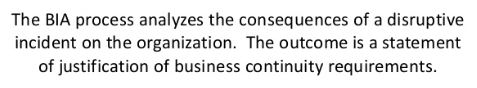
\includegraphics[width=12cm]{BIA.png}
\caption{Definizione di BIA secondo lo Standard ISO 22317 \href{https://www.slideshare.net/TheBCEye/isos-newest-standard-the-bia-iso-22317}{www.slideshare.net/}}
\end{figure}

Nella Business Impact Analysis viene svolta una analisi . In particolare ci si concentrerà sulla prioritizzazione di servizi, processi e attività, sulla base degli effetti o le conseguenze dell'interruzione delle funzioni aziendali IT critiche.
\\In una BIA si dovrebbero anche quantificare i costi associati a un disastro (perdite finanziarie o ripercussioni su relazioni pubbliche, morale, salute e sicurezza o perdita del vantaggio competitivo). Nel presente documento viene accennato il calcolo dei costi, che però dovrebbe essere complementato e completato in presenza di dati più esaurienti.
\\ La BIA deve essere stesa in stretta collaborazione col processo di Risk Management ed è un buon punto di partenza per la valutazione degli obiettivi del tempo di recupero (RTO) e gli obiettivi del punto di ripristino (RPO) e delle risorse e i materiali necessari per la continuità aziendale.
\vspace{0.5cm}
\\ Per la stesura della BIA, ci avvaleremo del corpo centrale del template \textbf{ISO 22317}.
\vspace{0.5cm}
\begin{figure}[H]
\centering
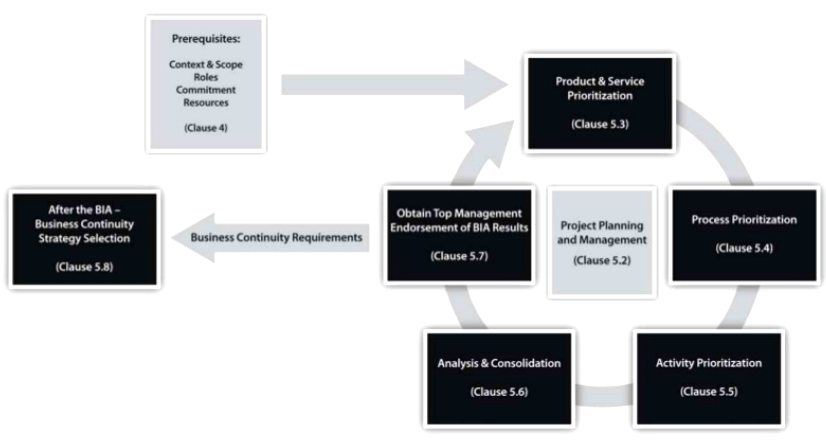
\includegraphics[width=12.5cm]{bia_schema.png}
\caption{Definizione di BIA secondo lo Standard ISO 22317\href{https://www.slideshare.net/TheBCEye/isos-newest-standard-the-bia-iso-22317}{www.slideshare.net/}}
\end{figure}

\newpage
\subsubsection{Product and Service Prioritization}
\begin{figure}[H]
\centering
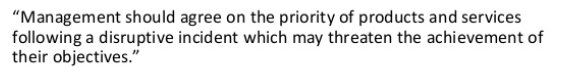
\includegraphics[width=12cm]{BIA_pes.png}
\caption{Definizione di Product and Service Prioritization\href{https://www.slideshare.net/TheBCEye/isos-newest-standard-the-bia-iso-22317}{www.slideshare.net/}}
\end{figure}
In questa sezione viene data una priorità ai servizi oggetto di appalto.\\
La priorità varia in una scala da 1 a 5 dove 1 indica una bassa priorità e 5 indica un'alta priorità.

\renewcommand\arraystretch{1,3}
\begin{longtable}{p{10cm} c}
\toprule
\textbf{Servizio} & \textbf{Priorità} \\
\toprule
Conduzione operativa dei sistemi di elaborazione & 5 \\
Pianificazione e controllo delle elaborazioni & 3 \\
Manutenzione degli ambienti software di sistema & 4 \\
Systems \& LAN Management & 4 \\
\hspace{2cm} tra cui servizio internet generale & 5 \\
\hspace{2cm} tra cui servizio internet dorsale & 4 \\
\hspace{2cm} tra cui servizio internet terminale & 3 \\
Call Center Interno & 3 \\
Gestione della configurazione & 3 \\
Outsourcing delle postazioni di lavoro & 3 \\
Manutenzione del software applicativo & 4 \\
Formazione & 3 \\
Servizio di housing & 5 \\
Servizio di supporto direzionale & 3 \\
Servizio di supporto gestione del personale & 3 \\
\bottomrule
\caption{BIA - Service Prioritization}
\end{longtable}

\newpage
\subsubsection{Process Prioritization}
\begin{figure}[H]
\centering
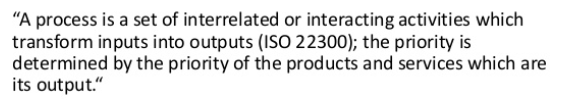
\includegraphics[width=12cm]{BIA_proc.png}
\caption{Definizione di Processo secondo lo Standard ISO \href{https://www.slideshare.net/TheBCEye/isos-newest-standard-the-bia-iso-22317}{www.slideshare.net/}}
\end{figure}
In questa sezione viene data una priorità ai processi dell'Istituto Gaetano Pini, comprendendo sia i processi che l'offrente andrà ad istanziare (come richiesto nel capitolato d'appalto in 5.1.4) sia i processi oggetto di rivisitazione, e descritti nel cap.1 del presente documento.\\
La priorità varia in una scala da 1 a 5 dove 1 indica una bassa priorità e 5 indica un'alta priorità.\\
\renewcommand\arraystretch{1,5}
\begin{longtable}{p{8cm} c}
\toprule
\textbf{Processo} & \textbf{Priorità} \\
\toprule
Asset management & 2 \\
Change management & 2 \\
Problem management & 3 \\
Business continuity & 3 \\
Misurazione dei livelli di servizio & 2 \\
Processo di gestione delle prestazioni ambulatoriali & 3 \\
Processo di gestione delle prestazioni di ricovero & 2 \\
Processo di gestione delle prestazioni di Pronto Soccorso & 5\\
\small{\hspace{1cm} tra cui operazioni coinvolgenti attività di codice giallo e rosso} & 5\\
\small{\hspace{0.5cm} tra cui operazioni coinvolgenti attività di codice bianco e verde e altre operazioni} & 4\\
Processo di gestione risorse economiche & 3 \\
Processo di gestione risorse umane & 2 \\
Processi di gestione direzionale & 2 \\
\bottomrule
\caption{BIA - Process Prioritization}
\end{longtable}

\newpage
\subsubsection{Activity Prioritization}
\begin{figure}[H]
\centering
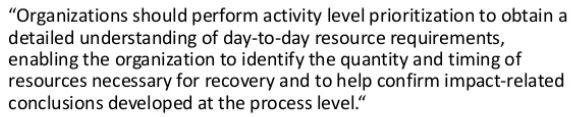
\includegraphics[width=12cm]{BIA_act.png}
\caption{Definizione di Activity Prioritization \href{https://www.slideshare.net/TheBCEye/isos-newest-standard-the-bia-iso-22317}{www.slideshare.net/}}
\end{figure}

In questa sezione viene data una priorità alle attività. Tutto ciò quello che viene definito come \textbf{attività} viene elencato nelle tabelle sottostanti di prioritizzazione delle attività (che partono dalla pagina successiva - per saltare le tabelle vedere in \ref{fineattprio}).\\
La priorità varia in una scala da 1 a 5 dove 1 indica una bassa priorità e 5 indica un'alta priorità.\\

\paragraph{Conduzione operativa dei sistemi di elaborazione}
\textcolor{white}{.} \\
\renewcommand\arraystretch{1,3}
\begin{longtable}{p{12cm} c }
\toprule
\textbf{Attività} & \textbf{Priorità} \\
\toprule
Accensione ed inizializzazione apparecchiature e sistemi, attivazione delle configurazioni (hardware e software)  & 4 \\
Controllo   dei   sistemi   e   del   corretto   funzionamento,   diagnosi   di   primo   livello   dei malfunzionamenti,  attivazione  dei  tecnici  delle  società  preposte  alla  manutenzione  e fornitura del relativo supporto  & 3 \\
Registrazione,   nel   sistema   di   gestione   dei   problemi,   dei   malfunzionamenti   delle 
apparecchiature,della relativa diagnosi, dei conseguenti interventi di ripristino e dello stato degli interventi & 2 \\
Attivazione  e  controllo  elaborazioni  batch  e/o  stampe,  secondo  le  schedulazioni previste,  & 2 \\
Montaggio/smontaggio dei supporti sulle unità di registrazione & 2 \\ 
Attivazione di procedure di salvataggio delle informazioni e delle applicazioni (back up e disaster recovery)  
 & 5 \\
Registrazione delle attività ed elaborazione di statistiche di consuntivo sulla operatività e disponibilità delle apparecchiature e dei sistemi condotti.  & 2 \\
Tenere un giornale delle attività e dei problemi &2 \\
Tenere un riepilogo periodico consuntivo del periodo di osservazione concordato con l’Istituto, che riporti  statistiche  su  operatività  dei  sistemi  e  problemi. & 2 \\
\bottomrule
\caption{BIA - Activity Prioritization - Conduzione operativa dei sistemi di elaborazione}
\end{longtable}

\newpage
\paragraph{Pianificazione e controllo delle elaborazioni}
\textcolor{white}{.} \\
\renewcommand\arraystretch{1,5}
\begin{longtable}{p{11cm} c }
\toprule
\textbf{Attività} & \textbf{Priorità} \\
\toprule
Raccolta delle esigenze relative alle elaborazioni applicative periodiche  & 2 \\
Predisposizione  di  piani  di  lavoro  periodici  (giornalieri,  settimanali,  mensili,  ecc.)  per  le procedure pianificate (es. stampe cedolini, generazione flussi istituzionali, ecc.)  & 3\\
Ricezione e accodamento  richieste  di  attivazione  procedure,  non  pianificate,  e  schedulazione  delle procedure  & 3 \\
Controllo  della  corretta  esecuzione  delle  elaborazioni,  diagnosi  di  primo  livello  dei 
problemi  relativi  alla  esecuzione  di procedure  applicative,  attivazione  dei  tecnici  preposti alla risoluzione e loro supporto  & 3 \\
Registrazione delle attività, dei problemi, degli interventi di correzione anche nel sistema di gestione dei problemi,  & 2 \\
Elaborazione di statistiche di consuntivo  & 2\\
Tenuta di piani di elaborazione, comprensivi delle registrazione delle richieste  & 2\\
Tenuta di  un giornale delle attività effettuate con evidenza di quelle portate a termine correttamente, dei problemi e delle azioni correttive & 2 \\
Tenuta di  un  riepilogo  periodico  consuntivo,  almeno  trimestrale,  che  riporti  statistiche  su  attività  e problemi.  & 2 \\
\bottomrule
\caption{BIA - Activity Prioritization - Pianificazione e controllo delle elaborazioni}
\end{longtable}

\newpage
\paragraph{Manutenzione degli ambienti software di sistema}
\textcolor{white}{.} \\
\renewcommand\arraystretch{1,5}
\begin{longtable}{p{11cm} c }
\toprule
\textbf{Attività} & \textbf{Priorità} \\
\toprule
Aggiornamento   periodico,   programmato   o   estemporaneo,   dei   prodotti   in   base   alle specifiche  di  rilascio  di  nuove  versioni  o  release  o  patch  da  parte  dei  produttori  sia  per correzione  che  per  miglioramento.  L’aggiornamento  avverrà  solo  a  valle  di  verifiche  di compatibilità  delle  nuove  versioni  nell’architettura  complessiva  del  sistema  informatico  e comunque con autorizzazione da parte dell’Istituto.  
 & 2 \\
Manutenzione  programmata  (inclusa  la  dismissione  per  le  soluzioni  obsolete  ed  escluse dall’architettura)  e  soluzione  di  problemi  \textit{estemporanei}  per  componenti  mal  funzionanti, con diagnosi di primo livello, intervento sulla configurazione e attivazione dei tecnici delle società produttrici o di assistenza specifica sul prodotto.    &4 \\
Test  e  collaudo  dell’operatività  dei  sistemi,  dopo  l’aggiornamento  o  l’intervento  di 
manutenzione,   prima   dell’entrata   in   produzione.   A   tal   fine,   come   già   dichiarato 
precedentemente, si dovrà prevedere la presenza di un ambiente  di test nell’architettura 
complessiva del sistema informatico.   &3 \\
Aggiornamento della configurazione in funzione delle modifiche apportate (di versione, di prodotto, ecc.) e registrazione delle attività    & 3 \\
Tenuta di piani periodici di aggiornamento e di manutenzione programmata degli ambienti software di sistema   &2 \\
Tenuta di un  giornale  delle  attività  effettuate  (interventi  programmati,  aggiornamenti  effettuati,  etc.) con evidenza  dei problemi e delle azioni correttive, dei collaudi effettuati prima del rilascio in produzione e delle modifiche effettuate sulla configurazione  & 0 \\
Tenuta di un  riepilogo  periodico  consuntivo,  almeno  trimestrale,  che  riporti  statistiche  su  attività  e problemi. & 2 \\
\bottomrule
\caption{BIA - Activity Prioritization - Manutenzione degli ambienti software di sistema}
\end{longtable}

\newpage
\paragraph{Systems \& LAN Management}
\textcolor{white}{.} \\
\renewcommand\arraystretch{1,5}
\begin{longtable}{p{11cm} c }
\toprule
\textbf{Attività} & \textbf{Priorità} \\
\toprule
Monitoraggio e gestione dei server, delle LAN e dei posti di lavoro (PdL) & 5 \\
Gestione delle password, dei profili utente e degli indirizzi IP per l’accesso dei PdL alle risorse di rete  & 3 \\
Controllo  centralizzato  sulla  gestione  dei  server,  dei  file  system,    dei   profili   utente, gestione remota delle procedure di backup/recovery dei server;  & 5 \\
Monitoraggio  dello  stato  di  funzionamento  delle  singole  componenti  attive  delle LAN, dei firewall e degli apparati di rete  & 3 \\
Rilevazione dei malfunzionamenti degli apparati di rete e la loro gestione, & 5 \\
Rilevazione del traffico, per individuare possibili aree di inefficienza, colli di bottiglia o sintomi di malfunzionamento;   & 3 \\
Software distribution management  & 3 \\
Configuration management & 3\\
Performances analisys & 2 \\
Stampa & 2 \\
\bottomrule
\caption{BIA - Activity Prioritization - Systems \& LAN Management}
\end{longtable}

\newpage
\paragraph{Call Center Interno}
\textcolor{white}{.} \\
\renewcommand\arraystretch{1,3}
\begin{longtable}{p{13cm} c }
\toprule
\textbf{Attività} & \textbf{P.tà} \\
\toprule
Assicurare la comunicazione tempestiva ed efficace con l’utenza & 2 \\
Provvedere all’accoglimento ed alla registrazione delle richieste di assistenza o rigettarle se non di competenza  &2 \\
Risolvere  i  problemi  più  ricorrenti,  di  non  elevata  complessità,  assistenza  agli  utenti  relativamente  alla  fruizione  dei  servizi  del   sistema  informativo,   assistenza  nell'uso appropriato delle funzioni messe a disposizione dal sistema informativo;  & 3 \\
Smistare  al  personale  del  Centro  di  Gestione  e  a  strutture  di  assistenza  specifiche  la risoluzione dei problemi non risolvibili al primo livello,  &2 \\
Controllare i processi di risoluzione attivati e verificarne gli esiti,  & 2\\
Rendicontare all’utente sullo stato dell’intervento e chiudere l’intervento alla risoluzione del problema e/o della richiesta,  & 2  \\
Analizzare  le  statistiche  sugli  interventi,  al  fine  di  identificare  i  fabbisogni  (anche  di formazione) e definire azioni di prevenzione dei problemi.  & 2 \\
rispondere a informazioni sui servizi erogati dal sistema informativo;  & 1 \\
rispondere a assistenza sull’uso dei servizi e delle applicazioni;  & 1 \\
rispondere a eventuali problemi riscontrati;  & 1 \\
effettuare attivazione, (ri)configurazione, sospensione di un servizio;  & 2 \\
fornire risorse informatiche.  &2 \\
sopperire a difetti e/o a malfunzionamenti dei programmi applicativi; & 2 \\
istruire  il  personale  specializzato  per  il  superamento,  la  correzione  o  l'aggiramento  di eventuali errori presenti nei programmi; & 3 \\
fornire  le  nuove  versioni  e  gli  aggiornamenti  del  software  applicativo  e  le  eventuali 
correzioni necessarie per il software di base e d’ambiente; & 3 \\
supportare la installazione di nuove versioni dei programmi o gli aggiornamenti dei software di base e d'ambiente; &2\\
supportare   l'esecuzione   operativa   delle   funzioni   per   quanto   non   espressamente 
documentato nella manualistica d'uso o di gestione, ovvero non opportunamente descritto in sede di addestramento; & 4 \\
dare  assistenza  sistemistica  e  consulenza  riguardo  all’utilizzo  del  software  di  base  ed applicativo e per la risoluzione dei diversi problemi di esercizio connessi al funzionamento delle apparecchiature o all’impiego delle funzionalità applicative. & 3 \\
Tenuta consuntivi &2 \\
\bottomrule
\caption{BIA - Activity Prioritization - Call Center Interno}
\end{longtable}

\newpage
\paragraph{Gestione della configurazione}
\textcolor{white}{.} \\
\renewcommand\arraystretch{1,5}
\begin{longtable}{p{11cm} c }
\toprule
\textbf{Attività} & \textbf{Priorità} \\
\toprule
identificazione  e  gestione  delle  componenti  (configuration  item)  e  dello  stato  delle 
componenti   &3 \\
definizione  delle  procedure  formali  di  modifica  della  configurazione  (responsabilità, 
attività, ecc.)   & 2 \\
controllo  della  configurazione  con  analisi  delle  esigenze  e  delle  richieste  di  modifica, 
registrazione delle modifiche effettuate, archiviazione dei dati relativi,  & 2 \\
valutazione periodica della completezza della configurazione rispetto ai requisiti definiti, & 2 \\
gestione dei rilasci ed installazioni delle versioni delle componenti  & 2 \\
produzione di rapporti periodici ed a richiesta sullo stato della configurazione. & 2 \\
\bottomrule
\caption{BIA - Activity Prioritization - Gestione della configurazione}
\end{longtable}

\newpage
\paragraph{Outsourcing delle postazioni di lavoro}
\textcolor{white}{.} \\
\renewcommand\arraystretch{1,5}
\begin{longtable}{p{11cm} c }
\toprule
\textbf{Attività} & \textbf{Priorità} \\
\toprule
Manutenzione   di   hardware   e   software   di   base   (preventiva,   adattativa,   correttiva), & 4 \\
Installazione di hardware e software, gestione delle modifiche e degli aggiornamenti.  & 3 \\
Gestione  dei  dati  e  delle  configurazioni  degli  utenti  (backup  e  restore,  installazione  e gestione  prodotti  antivirus,  installazione  e  gestione  applicazioni  per  servizi  internet  e 
posta);(l’onere del backup dei documenti e dei dati sulle postazioni, se non legati ad applicazioni centralizzate, resta a carico degli utenti stessi.)  & 3 \\
Gestione delle risorse critiche, con particolare attenzione alle performance ed ai tempi di ripristino;   & 5 \\
Predisposizione rapporti periodici di consuntivazione dei problemi, ed analisi della qualità del  servizio  reso  attraverso  rilevazione  (errori,  chiamate,  tempi  di  attesa,  soddisfazione utente, ecc.)  & 5 \\
\bottomrule
\caption{BIA - Activity Prioritization - Outsourcing delle postazioni di lavoro}
\end{longtable}

\paragraph{Manutenzione del software applicativo}
\textcolor{white}{.} \\
\renewcommand\arraystretch{1,5}
\begin{longtable}{p{11cm} c }
\toprule
\textbf{Attività} & \textbf{Priorità} \\
\toprule
Manutenzione correttiva &5 \\
Manutenzione adeguativa & 3 \\
Manutenzione normativa & 4 \\
Manutenzione migliorativa & 3 \\
Manutenzione evolutiva & 2 \\
Tenuta consuntivi & 2 \\
\bottomrule
\caption{BIA - Activity Prioritization - Manutenzione del software applicativo}
\end{longtable}

\newpage
\paragraph{Formazione}
\textcolor{white}{.} \\
\renewcommand\arraystretch{1,5}
\begin{longtable}{p{11cm} c }
\toprule
\textbf{Attività} & \textbf{Priorità} \\
\toprule
Tenuta lezioni & 3 \\
Tenuta verifiche & 2 \\
Tenuta consuntivi & 2 \\
\bottomrule
\caption{BIA - Activity Prioritization - Formazione}
\end{longtable}

\paragraph{Servizio di supporto direzionale}
\textcolor{white}{.} \\
\renewcommand\arraystretch{1,5}
\begin{longtable}{p{11cm} c }
\toprule
\textbf{Attività} & \textbf{Priorità} \\
\toprule
Analisi dei processi aziendali e dei principali flussi   & 3 \\
Supporto  alla  progettazione  del  sistema  e  dei  processi  per  il  controllo  di  gestione  ed  il budgeting  & 3 \\
Disegno del sistema informativo per  supportare adeguatamente i processi e la raccolta dei 
dati necessari per le funzioni di controllo  & 3 \\
Disegno del sistema di reporting sia in ambito amministrativo che sanitario  & 3 \\
Controllo correttezza dei flussi istituzionali (completezza dei dati raccolti, congruità, ecc.)  & 4 \\
Tenuta consuntivi & 0 \\
\bottomrule
\caption{BIA - Activity Prioritization - Servizio di supporto direzionale}
\end{longtable}

\newpage
\paragraph{Servizio di supporto gestione del personale}
\textcolor{white}{.} \\
\renewcommand\arraystretch{1,5}
\begin{longtable}{p{11cm} c }
\toprule
\textbf{Attività} & \textbf{Priorità} \\
\toprule
Gestione tabellare (aggiornamento dati relativi alle codifiche fondamentali e ai parametri da 
utilizzare nei calcoli e provenienti dalla indicazioni legislative e contrattuali) su indicazione 
del  responsabile  del  servizio  e  con  valutazione  delle  modifiche  indotte  da  variazioni 
legislative)  &4 \\
Cedolini, dichiarazioni, modulistica e in genere elaborati richiesti dalla normativa  & 3 \\
Reportistica standard  & 2 \\
Flussi verso altri sistemi aziendali  & 3 \\
Imbustamento, distribuzione e consegna cedolini con modalità proposta dalle ditte (in sede, 
via postel, etc.)  & 3\\
Gestione badge aziendali (consegna, sostituzione, ritiro, etc.)  & 2\\
Altri servizi di supporto,  proposti dalle ditte, aggiuntivi e ad integrazione di questi già citati.  & 2\\
\bottomrule
\caption{BIA - Activity Prioritization - Servizio di supporto gestione del personale}
\end{longtable}

\paragraph{Altri servizi}
\textcolor{white}{.} \\
\renewcommand\arraystretch{1,5}
\begin{longtable}{p{11cm} c }
\toprule
\textbf{Attività} & \textbf{Priorità} \\
\toprule
Firma digitale & 3 \\
Gestione documentazione & 2 \\
Gestione accesso ai dati & 4 \\
\bottomrule
\caption{BIA - Activity Prioritization - Altri servizi}
\end{longtable}

\newpage
\subsubsection{Analysis and Consolidation} 
\label{fineattprio}
In questa sezione, che deve essere stesa in stretta collaborazione col processo di Risk Management, cercheremo di dare delle linee guida una stima dell'impatto di un evento.\\
Per calcolare la stima degli impatti, useremo come base il modello indicato da \href{http://security.polito.it/~lioy/01jem/risk05_risk_2x.pdf}{security.polito}.
Un \textbf{evento} trae ispirazione, secondo quanto scritto nel capitolato) dai processi dell'Istituto, dai servizi offerti oggetto di appalto, dalle tipologie di prestazione sanitaria effettuate dall'Istituto e dalle fasi sanitarie descritte in ambito CRS-SISS. Segue una breve descrizione di questi punti citati.
\vspace{1cm}
\\
\textbf{Fasi sanitarie in ambito CRS-SISS}
\begin{itemize}
    \item prescrizione 
      \begin{itemize}
          \item identificazione cittadino - IdCitt
          \item prescrizione - Ps
      \end{itemize}
    \item accoglienza
        \begin{itemize}
           \item prenotazione (non presente in fase di pronto soccorso) - Pn
            \item pagamento -  \$
            \item accettazione (identificazione della prescrizione prenotata) - IdPs
         \end{itemize}
    \item erogazione 
        \begin{itemize}
          \item trasferimento (di reparto) - Tr
          \item dismissione - Dism
          \item messa a disposizione del referto - Ref
        \end{itemize}
    \item rendicontazione - Rend
 \end{itemize}
 \vspace{1cm}
 \textbf{Tipologie di prestazione sanitaria effettuate dall'Istituto}
  \begin{itemize}
  \item ortopedia e traumatologia
  \item recupero e riabilitazione funzionale
  \item reumatologia e servizi sanitari di supporto
  \item chirurgia vascolare
  \end{itemize}

\newpage
\paragraph{Moltiplicatore evento}
Per calcolare l'impatto di un evento useremo un apposito \textit{moltiplicatore evento}. La seguente tabella è una tabella ausiliaria utile al calcolo del \textit{moltiplicatore evento}. 
Il moltiplicatore è un primo tentativo di riassumere le attività messe a rischio comprendono persone, proprietà, catena di fornitura, tecnologia informatica, reputazione aziendale e obblighi contrattuali, altrimenti difficilmente valutabili quantitativamente.
\renewcommand\arraystretch{1,2}
\begin{longtable}{p{4cm} c c c c c c c c c}
\toprule
\textbf{Tipologia} & IdCitt & Ps & Pn & \$ & IdPs & Ts & Dism & Ref & Rend \\
\toprule
Ortopedia e traumatologia (base +2) & +1 & 0 & 0 & 0 & 0 & -1 & -1 & -1 & -1 \\
Recupero e riabilitazione funzionale (base 0) & +1 & 0 & 0 & 0 & 0 & -1 & -1 & -1 & -1 \\
Reumatologia e servizi sanitari di supporto (base 0) & +1 & 0 & 0 & 0 & 0 & -1 & -1 & -1 & -1 \\
Chirurgia vascolare (base +1) & +1 & 0 & 0 & 0 & 0 & -1 & -1 & -1 & -1 \\
\bottomrule
\caption{BIA - Bonus fase e tipologia}
\end{longtable}

Per calcolare il moltiplicatore ci si affiderà alla seguente formula: 
\begin{center}
	\line(1,0){350}\\
    \vspace{0,1cm}
	\textit{Molt. evento} = (\textit{Priorità dell'attività}
    		+\textit{Bonus fase e tipologia})
            X \textit{Priorità processo}
	\line(1,0){350}
\end{center}
in cui la \textit{Priorità dell'attività} è data dalle tabelle sottostanti, il \textit{Bonus di fase e tipologia} è data dalla tabella sovrastante, e la \textit{Priorità del processo} è data dalla tabella della \textit{Priorità dei processi}.
\\ Se una attività comporta più conseguenze, in più fasi e/o tipologie e/o in più processi, si effettuerà la sommatoria di ogni conseguenza.
\\ Il \textit{Bonus di fase e tipologia} è da sommare alla \textit{Priorità dell'attività} solo nei casi in cui la classificazione dell'attività per fase e tipologia risulti sensata. I casi esatti saranno  definiti nella fase di progettazione esecutiva della soluzione oggetto di appalto. 

\begin{center}
	\line(1,0){350}
\end{center}
\begin{changemargin}{0.5cm}{0.5cm}
  \textbf{Esempio: accensione sistemi di prenotazione di visite ambulatoriali ortopediche:}\\
  Priorità dell'attività = 4 (accensione)\\
  Bonus di fase e tipologia = 2 (ortopedia e traumatologia Pn)\\
  Priorità del processo coinvolto = 3 (ambulatorio)\\
  \textbf{Moltiplicatore evento} = (4 + 2) x 3 = 18
\end{changemargin}
\begin{center}
	\line(1,0){350}
\end{center}

\paragraph{Stima degli impatti}
Per calcolare la stima degli impatti, useremo come base il modello indicato da \href{http://security.polito.it/~lioy/01jem/risk05_risk_2x.pdf}{security.polito}.\\
L'impatto di un evento (es: mancata accensione dei sistemi di prenotazione di visite ambulatoriali ortopediche) viene calcolato come:
\\
\begin{center}
	\line(1,0){350}
    \vspace{0,1cm}
\textit{impatto(evento)} = \textit{valore asset} X \textit{danno\%} X \textit{moltiplicatore evento}
	\line(1,0){350}
\end{center}
in cui:
\begin{itemize}
\item \textit{valore asset} è il valore dell'asset coinvolto direttamente nell'evento. Questo valore è da determinare in collaborazione con i processi di configuration management.
\item \textit{danno\%} è il valore in percentuale del danneggiamento;
\item \textit{moltiplicatore evento} è il numero calcolato al punto precedente.
\end{itemize}

\begin{center}
	\line(1,0){350}
\end{center}
\begin{changemargin}{0.5cm}{0.5cm}
  \textbf{Esempi:}
  \vspace{0.2cm}\\
  \textbf{Mancata accensione dei sistemi di prenotazione di visite ambulatoriali ortopediche:}\\
  Server Aurora = (es:500 000 euro) \\
  Danno\% = 0,01\% \\
  Moltiplicatore\% = 15 \\
  \textbf{Impatto} = (500 000 * 0,01\%) x 18 = 900 euro
  \vspace{0.2cm} \\
  \textbf{Mancata rilevazione dei malfunzionamenti al server di Aurora con conseguenze in pronto soccorso d'urgenza in fase di identificazione cittadino nell'area di traumatologia:}\\
  Server Aurora = (es:500 000 euro) \\
  Danno\% = 0,1\% \\
  Moltiplicatore\% = (5+3) * 5 = 40 \\
  \textbf{Impatto} = (500 000 * 0,1\%) x 40 = 20 000 euro
\end{changemargin}
\begin{center}
	\line(1,0){350}
\end{center}
Se un evento colpisce più asset, si effettuerà la sommatoria per asset. Questa analisi tuttavia non è esaustiva per molti aspetti. In fase di progettazione esecutiva dovranno essere considerati inoltre i seguenti aspetti:
\begin{itemize}
\item fattore tempo: la durata di tempo in cui si protrae il problema influsce nella stima degli impatti;
\item modalità di determinazione del danno in percentuale in modo esatto: deve essere stabilito con chiarezza chi ha il diritto/dovere di effettuare stime per questo dato;
\item modalità di determinazione dell'asset: in base alla definizione di asset, l'importo di questo dato può variare di molto (es: è asset l'intero SAP o i sono asset i suoi moduli?)
\end{itemize}
\vspace{1cm}
A quel punto, si potrà estrarre un elenco di eventi con quantificazione dell'impatto. Ai fini del progetto didattico ci limitiamo ad affermare che possiamo osservare che ci sono processi, attività e servizi che sono cruciali per il business dell'Istituto e che dovranno essere maggiormente soggette a protezione e controlli nella stesura della soluzione di continuità.

\newpage
\subsection{Criticità sistemi e applicativi}
\label{critsisapp}
Sulla base della Business Impact Analysis è possibile stendere la tabella delle criticità dei sistemi e applicativi. Per ognuno di questi si dovrebbe avere la lista dei CI correlati (nella documentazione stesa grazie alla collaborazione dei processi di Risk Management e del SACM), per poi assegnare una priorità ad ogni CI. Ai fini del progetto didattico si ritiene opportuno fermarsi alla tabella della criticità di sistemi e applicativi.

        \renewcommand\arraystretch{1.5}
        \begin{longtable}{c l c c c}
        \toprule
        \textbf{Ambito} & \textbf{Tecnologie} & \textbf{Criticità} \\
        \toprule
            \small{Urgenza, Ambulatorio e Degenza} & Aurora Web, ICAN &  5 \\
            %5 & Immagini & \small{RIS/PACS, AGFA/FUJI} & Dir. Img & 50 \\
             Emoderivati & SAP & 4 \\
             Analisi & PowerLab & 5 \\
             \small{Fatturaz., Archivio clinico, Referti} & SAP &  3 \\
            %4 & Punti gialli & NA & Dir. PtiGialli & ND\\
             SISS & ICAN & 3 \\
             Amministrazione & SAP & 2 \\
             \small{Ricoveri, Sale operatorie, Protesi} & SAP &  4 \\
             Gestione mail & SAP & 2 \\
             Gestione pazienti esterni & SAP  & 3 \\
             Gestione stampa & SAP & 2 \\
            \bottomrule
            \caption{Sistemi e applicativi della soluzione.}
        \end{longtable}


\newpage
\subsection{Valutazione dei rischi}
\label{rischi}
Lo scopo di questa sezione è quello di riportare alcuni dati che sarebbero in possesso del processo di Risk Management (e del SACM) che si occupa di identificare potenziali pericoli e valutare le sue le  vulnerabilità dell'Istituto rispetto ad esse.
\vspace{0.5cm} \\
Nella documentazione stesa grazie alla collaborazione dei processi di Risk Management e del SACM dovrebbero figurare, tra le varie, i CI che potrebbero essere messi in rischio. Ci dovrebbero essere quindi gli elenchi di hardware, software e dei dati critici e diagrammi che rappresentano le dipendenze tra essi. 
Il processo di Risk Management stabilirà come valutare questi dati (es. CRAMM) in suo possesso, in modo da rendere disponibile una stima più precisa dei livelli di rischio. Durante la fase di valutazione del rischio, i risultati della BIA possono essere esaminati rispetto a vari scenari di pericolo e le potenziali interruzioni possono essere prioritarie in base alla probabilità del rischio e alla probabilità di impatto negativo sulle operazioni commerciali.
\vspace{0.5cm} \\
Ai fini del progetto didattico si ritiene opportuno fermarsi alla tabella sottostante che mostra l'elenco dei rischi identificati con associati il livello di minaccia e di vunerabilità. Per ognuna delle seguenti voci sono state consultate fonti autorevoli (es. Terremoto: \href{https://www.thelocal.it/20161028/which-areas-of-italy-have-the-highest-risk-of-earthquakes}{thelocal.it}
\vspace{0.5cm} \\
Queste analisi verranno usate per giustificare gli investimenti in prevenzione e mitigazione, nonché la strategia di continuità che verrà identificata nelle pagine seguenti.
\newpage
\paragraph{Rischi}
\textcolor{white}{.} \\
\renewcommand\arraystretch{1,5}
\begin{longtable}{p{7cm} c c c }
\toprule
\textbf{Evento} & \textbf{Minaccia} & \textbf{Vulnerabilità}\\
\toprule
Terremoto & 1 & 2 \\
Allagamento & 3 & 3 \\
Uragano & 1 & 4 \\
Incendio & 4 & 1 \\
Interruzione dell'erogazione del servizio da parte del fornitore di SAP & 4 & 2 \\
"" "" di Aurora Web & 5 & 2 \\
"" "" di PowerLab & 4 & 2 \\
"" "" del SISS & 6 & 4 \\
Indisponibilità generica di corrente elettrica & 8 & 5 \\
Interruzione cablaggio dorsale & 3 & 4 \\
Interruzione cablaggio terminale & 2 & 3 \\
Attacco informatico (dati rubati) a SAP o Aurora o cache ICAN-SISS& 3 & 2 \\
Attacco informatico (dati rubati) a PowerLab& 2 & 2 \\
Attacco informatico (dati editati o cancellati) a SAP o Aurora o ICAN-SISS& 3 & 2 \\
Attacco informatico (dati editati o cancellati) a PowerLab& 2 & 2 \\
Attacco informatico (ddos o simili) a sistemi SAP o Aurora o ICAN-SISS& 3 & 2 \\
"" "" PowerLab & 2 & 2 \\
"" "" di ridondanza& 2 & 2 \\
Indisponibilità di persone chiave & 4 & 3 \\
\bottomrule
\caption{BIA - Valutazione dei rischi}
\end{longtable}


\newpage
\subsection{Identificazione RTO e RPO}
\label{rtorpo}
L'RPO (RecoveryPoint Objective) è la perdita dati tollerata (in tempo) mentre l'RTO (RecoveryTime Objective) è il tempo di ripristino servizio. La seguente figura mostra graficamente e dà una definizione formale di questi due termini. \\ Si riportano gli RTO e gli RPO per ogni applicativo/sistema risultanti dall'analisi effettuata tramite BIA, prioritizzazione sistemi e applicativi e prioritizzazione rischi.

\begin{figure}[H]
\centering
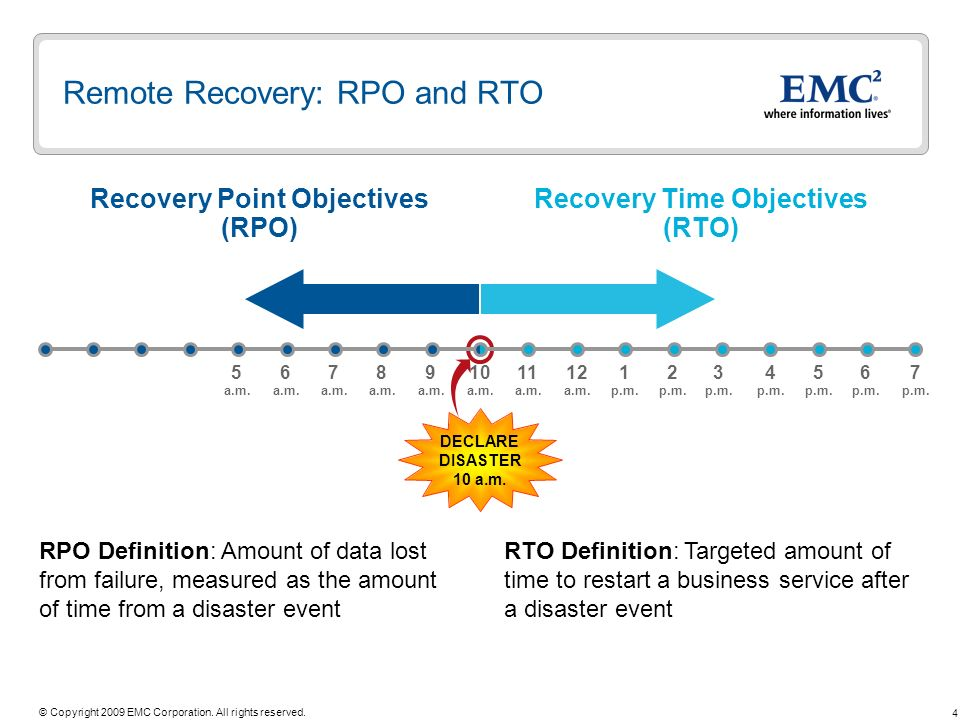
\includegraphics[width=14cm]{RPORTOdef.jpg}
\caption{Tempo e costo di recovery \href{https://slideplayer.com/slide/231966/}{slideplayer}}
\end{figure}

\renewcommand\arraystretch{1,5}
\begin{longtable}{p{5cm} p{2.5cm} c c }
\toprule
\textbf{Applicativo o sistema} & \textbf{Tecnologia} & \textbf{RTO} & \textbf{RPO} \\
\toprule
	Urgenza & Aurora Web & 15 minuti & 4 ore \\
    Ambulatorio & Aurora Web &4 ore & 4 ore \\
	Degenza & Aurora Web & 3 giorni & 8 ore \\
	Emoderivati & SAP & 8 ore & 8 ore \\
    Analisi & PowerLab & 1 ora & 8 ore \\
    Fatturazione & SAP & 1 settimana & 8 ore\\
    Archivio clinico & SAP & 1 settimana & 3 giorni\\
    Referti & SAP & 1 settimana & 3 giorni\\
    SISS & ICAN & 8 ore & 8 ore\\
    Direzione & SAP & 1 settimana & 8 ore\\
    Risorse umane & SAP & 1 settimana & 8 ore\\
    Ricoveri & SAP & 1 settimana & 8 ore\\
    Sale operatorie & SAP & 3 giorni & 4 ore\\
    Protesi & SAP & 3 giorni & 8 ore\\
    Mail & SAP & 8 ore & 4 ore\\
    Pazienti esterni & SAP & 8 ore & 8 ore\\
    Stampa & SAP & 1 settimana &  1 settimana\\
\bottomrule
\caption{RTO e RPO }
\end{longtable}







































%*******************************************************
\newpage
\section{Strategy Definition}
Sulla base della BIA, del Risk Assessment e degli RTO e RPO concordati, viene definita la strategia di continuità IT, con l'obbiettivo di di raggiungere l'equilibrio ottimale tra la minimizzazione del rischio e la razionalizzazione costo di gestione della continuità.\\

\subsection{Le opzioni}
Sono possibili 7 possibilità, dette Tier. La seguente tabella illustra i principali Tier, mostrando i relativi tempi di RTO e RPO. Il grafico mostra le riassume, mostrando la relazione tra costi e tempo di recovery per ogni tier.

\renewcommand\arraystretch{1,5}
\begin{longtable}{p{3,5cm} p{6,5cm} p{1,5cm} p{1,5cm} }
\toprule
\textbf{Tier} & Descrizione & RTO & RPO \\
\toprule
Tier-2: Data backup with a hot site &
regular backups on tape + hot site &
> 3 g. & 1-2 g. \\
Tier-3: \hspace{2cm} Electronic vaulting &
regular backups on tape + hot site + some data is electronically vaulted &
1g-3g. & <= 1g. \\
Tier-4: \hspace{2cm} Point-in-time copies &
more disk based solution (greater frequency) &
4h - 1g. & <= 4h \\
Tier-5: Transaction integrity
& synchronous data copy, atomic transaction &
1h-4h & <= 5min \\
Tier-6: \hspace{2cm} Siti paritetici &
mirroring of data to a remote server - solution independent from the SW used &
<= 1h & real time \\
\bottomrule
\caption{I 7 tier}
\end{longtable}

\begin{figure}[H]
\centering
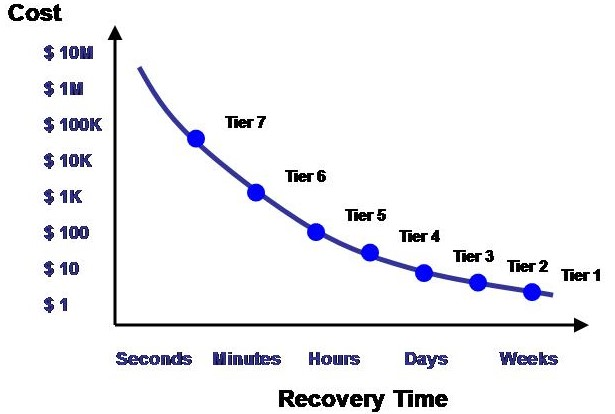
\includegraphics[width=12cm]{time345.jpg}
\caption{Tempo e costo di recovery \href{https://carlgusler.wordpress.com/2008/05/07/seven-levels-of-disaster-recovery-protection/}{carlgusler.wordpress.com}}
\end{figure}

\subsection{I tier richiesti}
In base alle tabelle precedenti possiamo ricavare i Tier richiesti per ogni applicativo/sistema.
\renewcommand\arraystretch{1,5}
\begin{longtable}{p{4cm} c c c c }
\toprule
\textbf{Applicativo o sistema} & \textbf{Tier} & \textbf{Tecnologia} & \textbf{RTO} & \textbf{RPO} \\
\toprule
	Urgenza 		& \textbf{5} & Aurora Web & 30 minuti & 60 minuti \\
    Ambulatorio		& 4 & Aurora Web &4 ore & 4 ore  \\
	Degenza 		& 3 & Aurora Web & 3 giorni & 8 ore \\
	Emoderivati 	& 4 & SAP & 8 ore & 8 ore \\
    Analisi 		& \textbf{5} & PowerLab & 1 ora & 4 ore \\
    Fatturazione 	& 3 & SAP & 1 settimana & 3 giorni \\
    Archivio clinico & 3 & SAP & 1 settimana & 3 giorni \\
    Referti 		& 3 & SAP & 1 settimana & 3 giorni \\
    SISS 			& 4 & ICAN & 8 ore & 4 ore \\
    Direzione 		& 3 & SAP & 1 settimana & 8 ore \\
    Risorse umane 	& 3 & SAP & 1 settimana & 8 ore \\
    Ricoveri 		& 3 & SAP & 1 settimana & 8 ore \\
    Sale operatorie & 4 & SAP & 3 giorni & 4 ore \\
    Protesi 		& 4 & SAP & 3 giorni & 4 ore \\
    Mail 			& 3 & SAP & 8 ore & 8 ore \\
    Pazienti esterni & 4 & SAP & 8 ore & 4 ore \\
    Stampa 			& 3 & SAP & 1 settimana &  1 settimana \\
\bottomrule
\caption{RTO e RPO }
\end{longtable}

\subsection{La scelta}
Per una scelta pienamente completa e consapevole, si dovrebbero avere dati riguardo i costi di avviamento e sostenimento delle varie soluzioni. Al fine del progetto didattico, ipotizziamo che, date le sostanziali risorse economiche e fisiche richieste per implementare il tier 4, e visti costi e benefici per l'implementazione dell'aggiuntivo tier 3, si ritiene opportuno utilizzare le infrastrutture e tecnologie usate per i servizi ospedalieri coperti da tier 4 anche per i servizi ospedalieri che in realtà richiederebbero solo un tier 3. In questo modo i costi di attivazione e mantenimento del tier 4 viene ripartito tra più servizi ospedalieri.
Riassumendo la soluzione è la seguente:
\renewcommand\arraystretch{1,5}
\begin{longtable}{p{4cm} c c c }
\toprule
\textbf{Tecnologia} & \textbf{Tier} & \textbf{RTO} & \textbf{RPO} \\
\toprule
	Aurora Web 	& 5 & 30 minuti & 60 minuti \\
    PowerLab 	& 5 & 1 ora 	& 4 ore \\
    SISS 		& 4 & 8 ore 	& 4 ore \\
	SAP 		& 4 & 8 ore 	& 4 ore\\
\bottomrule
\caption{RTO e RPO - Tecnologie e tier}
\end{longtable}

\subsection{Tempi e modalità di realizzazione della soluzione}
\label{ScadenzaContinuità}
L'implementazione delle soluzioni in modo completo e funzionanete, verrà realizzata nell'arco di 34 mesi per il Tier 4, mentre di 28 mesi per il Tier 5. Tuttavia tutta una serie di sistemi secondari potranno essere pronti prima di tale data, in modo concorde all'avanzamento dei lavori nel progetto, con possibilmente soluzioni di carattere temporaneo. La soluzione di continuità riguarda in ogni caso servizi e sistemi da noi erogati, iscritti in progetto.
\renewcommand\arraystretch{1,3}
\begin{longtable}{p{3cm} p{6cm}}
\toprule
\textbf{Tier} & \textbf{Tempo di realizzazione} \\
\toprule
    Tier 4 & 30 mesi \\
    Tier 5 & 24 mesi \\
\bottomrule
\caption{Tempi di realizzazione}
\end{longtable}

Segue il diagramma di Gantt con la schedulazione dei task ad alto livello da mettere in atto per la realizzazione della soluzione. Il diagramma rappresenta i task ad alto livello.

\begin{figure}[H]
\centering
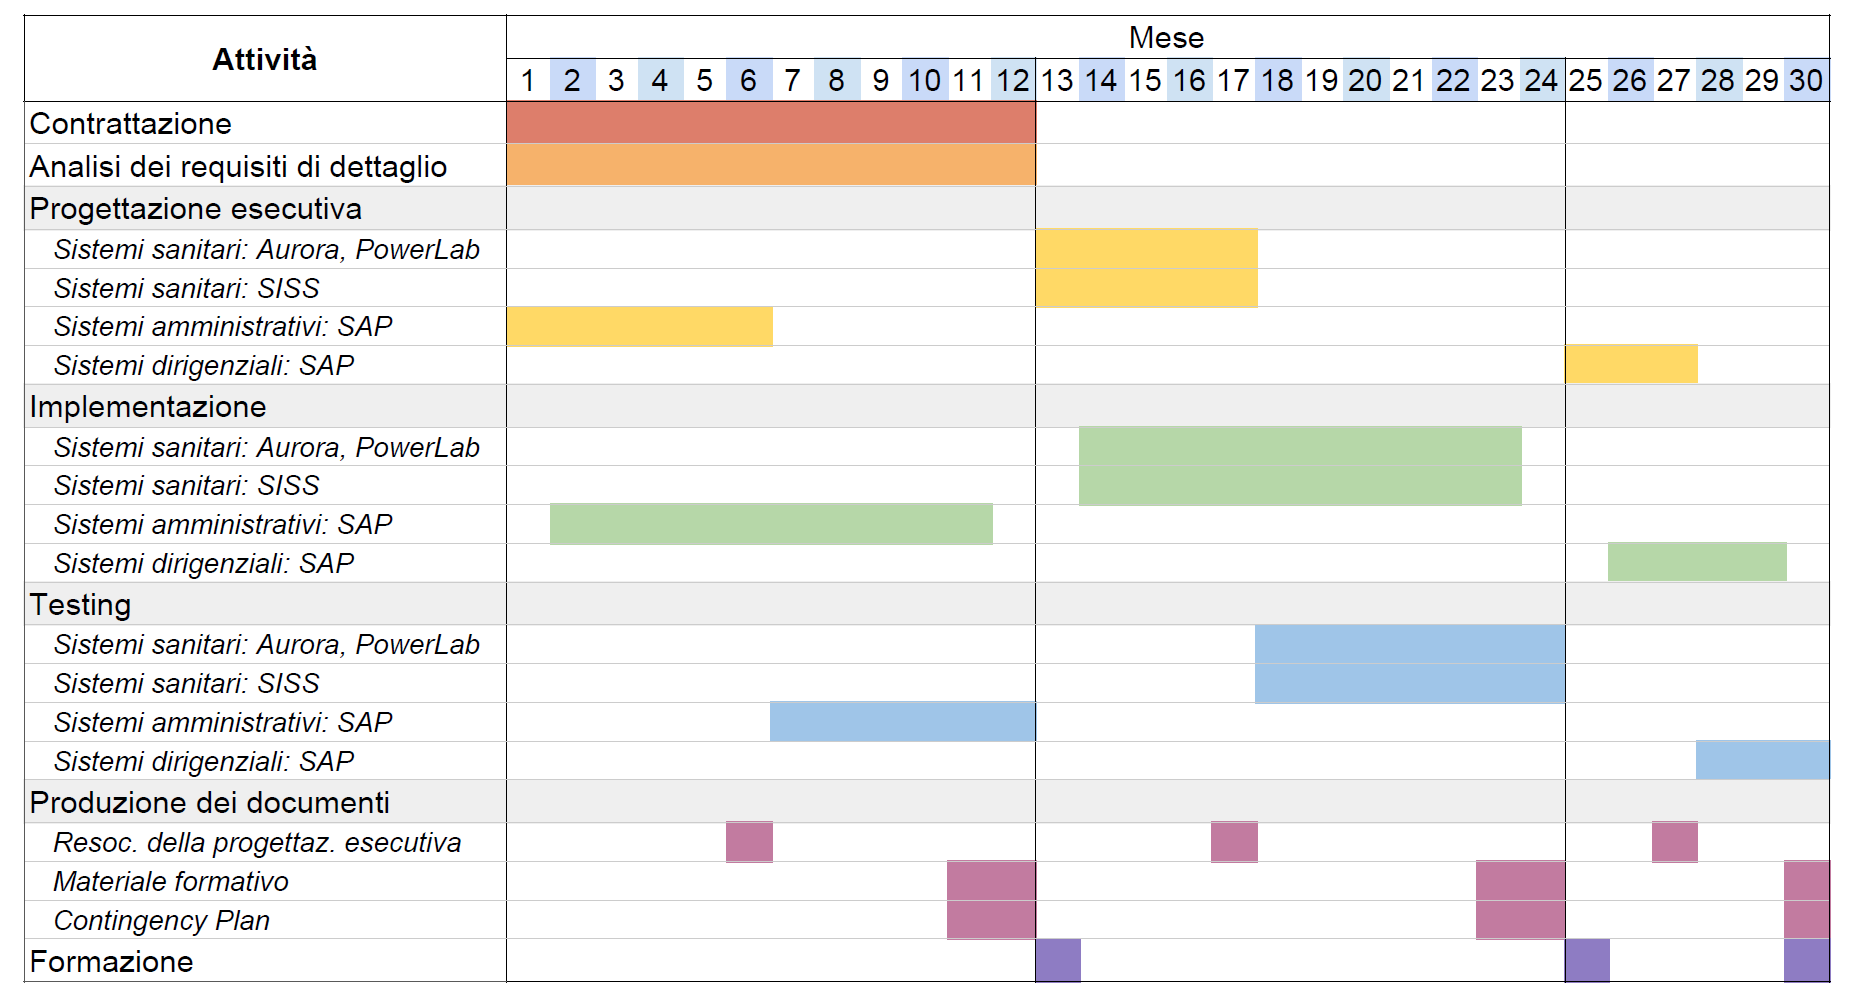
\includegraphics[width=14cm]{gantt-cont.PNG}
\caption{Diagramma di Gantt per la Continuità}
\end{figure}

\subsection{Trasferimento dati tra i siti}
\subsubsection{Caricamento iniziale dei dati}
In fase di caricamento iniziale dei dati nel sito secondario e in fase di rientro presso il sito primario, potranno essere usate anche soluzioni off-line. Una stima sommaria dei dati variati a livello giornaliero indica un ordine di grandezza di decine di TB. Per una stima dettagliata si dovrebbe avere il parere del Capacity Management.
\\Il trasferimento dati può essere relativo a dati sensibili. Vedere la sezione relativa in \ref{cap:rolloutplan}.
\subsubsection{Trasmissione periodica dei dati variati} In considerazione:
\begin{itemize}
\item dei volumi di dati ipotizzati;
\item della distribuzione oraria della finestra di produzione degli aggiornamenti dei dati operati dai servizi oggetto di 
soluzione, concentrata sostanzialmente nella fascia oraria 9.00 – 18.00 dei giorni feriali;
\item del valore di RPO previsto per i servizi oggetto di
 soluzione, variabile tra 60 minuti, 4 ore, 8 ore (e oltre)
\end{itemize}
E' prevista la trasmissione on-line dei dati variati. Parametri di disponibilità, velocità di trasferimento e sicurezza (sia della linea, sia delle caratteristiche dipendenti dalla quantità di dati da trasportare), verranno determinati con maggiore certezza e grado di dettaglio in sede di progettazione esecutiva in collaborazione col Capacity Management. Una stima sommaria dei dati variati a livello giornaliero indica un volume orientativo di alcune centinaia di GB. Al momento si ipotizza una banda di 100Mbps.\\ 	\\
La periodicità degli back-up sarà \textbf{almeno giornaliera} per tutti i servizi, con meccanismi automatici. 
Vedere la sezione di implementazione in \ref{implementation} per maggiori dettagli.
% \begin{itemize}
% \item Per i sistemi \textbf{SISS}, \textbf{PowerLab} e \textbf{ICAN} è previsto almeno un ulteriore salvataggio, da stabilire in sede di progettazione esecutiva. Ad ora si ipotizza un salvataggio aggiuntivo indicativamente a metà giornata lavorativa, per venire incontro ai requisiti di RPO esposti in precedenza.
% \item Per \textbf{Aurora Web} verrà ipotizzata una soluzione ad-hoc viste le prioritizzazioni dei processi e servizi associati a tale tecnologia, che garantisca il soddisfacimento dei requisiti richiesti.
% \end{itemize}
% La banda garantita sarà condivisa tra i servizi distribuendo gli eventi di aggiornamento in modo da evitare conflitto nell’accesso alla risorsa. 
% \\Il trasferimento dati può essere relativo a dati sensibili. Vedere la sezione relativa in \ref{cap:rolloutplan}.

\subsection{Risorse elaborative nel sito primario}
Il tipo di risorse elaborative nel sito primario è misto. 
Sono presenti sia infrastrutture di tipo virtuale che fisico. Il processo di SACM si occuperà di elencare in modo dettagliato i CI presenti nel sito primario.

\subsection{Risorse elaborative previste nel sito secondario}
In coerenza con il Tier 4 individuato, la soluzione prevede che le risorse elaborative nel sito secondario siano sempre disponibili e coerenti con quelle del sito primario, permettendo la ripartenza delle funzionalità in tempi rapidi.\\ 
Le risorse elaborative nel sito secondario saranno basate su una 
infrastruttura hardware in grado di operare su un 
numero di server virtuali sufficienti ad assolvere alle
esigenze di elaborazione del sito primario, completate
da un pool di macchine fisiche volte a raccogliere le
esigenze elaborative non coperte da ambienti virtuali.Si prevede 
la virtualizzazione dei desktop in modo da offrire posti 
di lavoro fruibili localmente o via VPN.
Un dimensionamento preciso verrà effettuato in fase di progettazione esecutiva.


\subsection{Storage, connettività e numero di Postazioni di Lavoro (PdL)}
Gli storage dei siti primari a livello di server hanno dimensioni nell'ordine di decine di TB. Presso il sito secondario si prevedono risoprse tra il 75 e il 100\% dei TB presenti nel sito primario.
\\ E' garantita la copertura di rete nel sito secondario. La banda esatta verrà determinata in sede di progettazione esecutiva.
\\ Nel sito secondario si prevede un numero di PdL utilizzabili 
prevalentemente per attività di back office in numero ridotto 
rispetto a quanto presente nella sede di normale operatività (tra 400 e 500). Il numero esatto verrà stabilito in sede di progettazione esecutiva, ma al momento si stima un numero di PdL compreso tra 30 e 80. Le modalità e i tempi di approvvigionamento e operatività delle risorse in linea di massima sono deducibili dal Gantt soprariportato.
L'Offerente si preoccuperà di descrivere la rete interna (cablaggio, router, switch, firewall, ecc.).
%todo Descrizione della rete interna (cablaggio, router, switch, firewall, ecc.)

\subsection{Localizzazione della struttura di continuità IT}
I  principali  fattori  che  sono stati valutati  nella  scelta  della  localizzazione  del sito secondario  sono  i seguenti:
\begin{itemize}
\item fattori geo-climatici;
\item disponibilità di infrastrutture per le telecomunicazioni;
\item impatto del fattore distanza/vicinanza;
\end{itemize}
E' stata scelta la struttura X in via Y n. Z a Cremona come struttura di continuità IT.
La struttura sarà adatta alle \hyperref{https://www.agid.gov.it}{linee guida Agid} per quanto riguarda:
\begin{itemize}
\item pavimenti e solai;
\item sistemi di illuminazione;
\item cablaggi e telecomunicazioni;
\item armadi e rack;
\item sistemi di raffreddamento e climatizzazione
\item alimentazione e continuità elettrica;
\item antincendio e anti-allagamento.
\end{itemize}

\subsection{Accessi fisici al sito secondario}
Al sito si accederà sia partendo dall'Istituto che partendo dalla sede dell'Offerente tramite automobile e autostrada. Nel retro dello stabile è disponibile un parcheggio gratuito, e affianco un parcheggio a pagamento.
\\
Per accedere fisicamente al sito secondario servono le autorizzazioni scritte (cartacee o elettroniche) dell'IT SC Manager (o del Vice SC Manager) o di un membro dell'IT SC Team.

\subsection{Personale all'interno della struttura secondaria in modalità standard}
Sarà presente fisicamente un operatore designato dall'Offerente a tenere controllato il sito secondario in orario 9-13 e 14-18. L'operatore non necessita di permessi per l'accesso fisico al sito secondario. La lista di operazioni, azioni e responsabilità a suo carico sono da definire con maggiore dettaglio in sede di progettazione esecutiva. Un esempio di operazione potrebbe essere la verfica dell'allineamento dei dati tra le due strutture a campione manualmente almeno una volta al giorno.

\subsection{Work-around manuali}
\label{workaround}
La soluzione individuata come Tier-4 potrebbe portare alla perdita dei dati prodotti nelle ore precendenti allo stato di emergenza, e potrebbe portare alla indisponibilità dei servizi per alcune ore dopo la dichiarazione dello stato di emergenza. Questi dati sono da considerare \textbf{persi} ai fini della soluzione di continuità aziendale. \\ Tuttavia per tentare di arginare i disagi dovuti a questo, si individuerà una serie di work-around manuali di modo che i processi ospedalieri possano continuare anche in situazione di emergenza, previa collaborazione del personale. Alcuni esempi possono essere individuati nella seguente lista, altri dettagli potranno essere aggiunti in fase di progettazione esecutiva.
\begin{itemize}
\item l'offerente si occuperà dell'hosting di una cartella condivisa tra tutti i dipendenti dell'Istituto;
\item all'interno della cartella ci saranno fogli di lavoro pre-impostati da definire con maggiore dettaglio in fase di progettazione esecutiva;
\item ogni dipendente dell'Istituto deve essere dotato di uno smartphone con connessione 3g e con accesso configurato alla cartella condivisa;
\item dal momento di dichiarazione dello stato di emergenza ogni dipendente è invitato a riportare ogni azione e operazione eseguita all'interno dei sistemi informatici nelle ultime quattro ore antecedenti alla dichiarazione;
\item per la gestione dei processi ospedalieri si farà riferimento, oltre che ai dati disponibili nei sistemi ordinari, anche alle informazioni trascritte nei fogli di lavoro suddetti.
\end{itemize}

\subsection{Doppiaggio linea telefonica, elettrica, internet}
Per ovviare ai disagi più comuni di interruzione di fornitura di corrente elettrica, linea telefonica o internet, è previsto di stilare contratti con fornitori terzi (diversi da quelli standard) appositamente per garantire un livello di continuità, seppur ridotto, sufficiente alla conduzione dei processi ospedalieri più importanti.
Si valuteranno attentamente alternative sia di prezzo ma soprattutto di modalità: collegamenti radio (es: Eolo), via terra o con altri mezzi). Si deve grantire un sistema di generazione e distribuzione dell’energia elettrica ridondato. La logica  di  ridondanza  si  deve  avvalere  di  apparecchiature  quali  UPS,  batterie  tampone,  gruppi elettrogeni  a  garanzia  della  continuità  di  erogazione  a  fronte  di  guasti  della  rete  di  distribuzione primaria. 

\subsection{Variazioni nei processi e servizi in fase di emergenza}
\begin{itemize}
\item \textbf{Formazione:} le attività del processo  di formazione vengono sospese fino al rientro completo dalla fase di emergenza;
\item \textbf{Documentazione:} le attività di documentazione e reporting richieste potranno subire dei ritardi; ad ogni modo ci si aspetta che al rientro vengano completati i documenti e i report richiesti entro un mese. Al rientro dalla situazione di emergenza, come previsto in \textit{Operational Management} in \pageref{rientro} si deve stilare un report sull'emergenza avvenuta.
\item \textbf{Service Level Management:} gli SLA in situazione di emergenza non subiranno variazioni;
\item \textbf{Change Management:} potranno essere aperte emergency-RFC in situazione di emergenza. Sarà poi competenza del processo di Change Management stabilire come gestire le emergency-RFC in emergenza in modo da garantire il bilanciamento tra tempi rapidi di risposta e sicurezza e correttezza nel cambiamento;
\item \textbf{Problem Management e Call Center Interno:} Il call center interno potrebbe essere ridotto in quanto a numeri del personale (perlomeno in fase di reazione all'emergenza). E' compito della funzione del Service Desk valutare se riorganizzare le procedure in situazione di emergenza, in modo da garantire il bilanciamento tra velocità e qualità di risposta;
%\item \textbf{Configuration Management:} 
\item \textbf{Processi ospedalieri: } per la gestione dei processi ospedalieri si farà riferimento, oltre che ai dati disponibili nei sistemi ordinari, anche alle informazioni trascritte nei fogli di lavoro suddetti in \ref{workaround}.
\end{itemize}


















































%*******************************************************
\newpage
\section{Implementation}
\label{implementation}

Sulla base della strategia concordata, viene pianificata l'implementazione, coinvolgendo i team IT nella parte di maggior dettaglio.
In questa fase sono previste:
\begin{itemize}
\item ulteriori analisi di dettaglio;
\item progettazione ad alto livello della soluzione di continuità;
\item progettazione esecutiva con sviluppo dei piani implementativi di dettaglio;
\item implementazioni di eventuali misure temporanee;
\item implementazione delle contromisure per la riduzione del rischio e dell'impatto. In particolare il Risk Management metterà in atto tutta una serie di contromisure preventive per i rischi identificati, quali incendi, allagamenti (es: posizionamento porte tagliafuoco, armadi appositi, ventole, raffreddamento).
\item testing.
\end{itemize}

Segue la progettazione ad alto livello della soluzione di continuità divisa per macro-tecnologia.

\newpage
\subsection{Soluzione di Continuità per Aurora Web e PowerLab}
\subsubsection{Interrelazioni con entità esterne all’Amministrazione}
I contratti in essere che vengono coinvolti sono:
\renewcommand \arraystretch{1,5}
\begin{longtable}{c c c}
\toprule
\textbf{Contratto in Essere} & \textbf{Fornitore} & \textbf{Produttore} \\
\toprule
	Contratto unico per fornitura servizi IT & Offerente & Offerente \\
\bottomrule
\caption{Contratti Aurora Web e PowerLab}
\end{longtable}
Non si rilevano necessità di effettuare variazioni contrattuali ai contratti sopracitati.

\subsubsection{Soluzione}
Per Aurora Web e PowerLab è prevista l'adozione del Tier 5.
\begin{figure}[H]
\centering
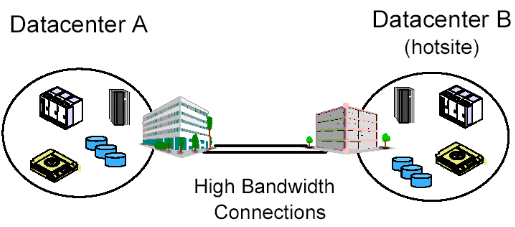
\includegraphics[width=8cm]{tier5.png}
\caption{Tier 5 \href{https://www.abzsol.com/cms/images/stories/pdf/business_continuity.pdf}{www.abzsol.com}}
\end{figure}
Sono previsti:
\begin{itemize}
\item backup off-site radicale ogni sei mesi su nastro da conservare presso l'\textit{Offerente};
%\item backup off-site incrementale una volta al giorno su disco da conservare presso l'hot site;
\item software di gestione Disaster Recovery (da stabilire in progettazione esecutiva es: Tivoli IBM);
%\item piano di Disaster Recovery di dettaglio da stilare in fase di progettazione esecutiva; 
\item hot-site con installazione del server di Aurora Web e PowerLab (con relative librerie e documentazione).
\end{itemize}
I due siti (primario e secondario) sono sincronizzati utilizzando una high-band connession. Gli aggiornamenti ai dati relativi ad Aurora saranno applicati in modo automatizzato sia al server locale, sia al server remoto, usando \textit{single-commit scope} che garantisce che i dati sul sito remoto e sul sito primario vengono aggiornati o retrocessi come un'unica unità di lavoro (UOW). I dati critici e le applicazioni sono quindi presenti su entrambi i siti e vengono persi solo i dati in transizione durante un disastro.\\
Altri dati necessari per eseguire l'applicazione (librerie, documentazione, copie delle licenze software) vengono inviati anche al sito secondario attraverso il software di gestione del DR al momento della creazione della soluzione. Il software permetterà anche il monitoraggio e il controllo della situazione in ogni momento sia antecedente all'emergenza, sia in fase di emergenza, che di rientro.

\subsubsection{Fase di reazione all’emergenza}
Istruzioni operative del start-up di dettaglio verranno fornite in sede di progettazione esecutiva. Si cercherà di automatizzare al massimo ogni operazione tramite script automatici, di modo da minimizzare, per quanto possibile, l'intervento umano. 
Supponendo che strutture generali, infrastruttura e componenti hardware siano ripristinati, le procedure di recupero rispetteranno le seguenti linee guida generali:
\begin{itemize}
\item avvio dei sistemi nel sito secondario tramite software di gestione del DR;
\item lancio della riconfigurazione automatizzata delle risorse di rete;
\item controllo del corretto collegamento del sistema alla rete di produzione;
\item controllo del corretto ripristino dei sistemi operativi;
\item  controllo del corretto ripristino della configurazione dei dati di sistema;
\item controllo del corretto ripristino del software applicativo;
\item  controllo del corretto ripristino dei dati applicativi;
\item lancio del testing automatizzato per la sicurezza;
\item lancio del testing automatizzato per le funzionalità di base del sistema;
\end{itemize}

\subsubsection{Fase di gestione dell’emergenza}
\begin{itemize}
\item L'amministrazione e monitoraggio dei sistemi di sostituzione per il sistema di Aurora viene affidato all'ing. X, e in secondo luogo al sig. XX.
\item L'amministrazione e monitoraggio dei sistemi di sostituzione per il sistema di PowerLab viene affidato all'ing. Y, e in secondo luogo al sig. YY.
\item Non è previsto che gli operatori sanitari, amministrativi, o che i tecnici debbano spostarsi fisicamente verso la struttura sostitutiva.
\item La situazione sarà sempre controllabile da remoto sia dall'Istituto che dalla \textit{nostra} azienda.
\item In caso di necessità è prevista la possibilità di mandare tecnici della \textit{nostra} azienda o professionisti esterni mandati da parte della nostra azienda.
\item Gli accessi ai sistemi Aurora dovranno essere controllati dal software di gestione di DR.
\item I dati creati in fase di gestione dell'emergenza devono essere memorizzati in un ambiente secondario, in modo da facilitarne il successivo restore.
\end{itemize}

%*******************************************************
\newpage
\subsection{Soluzione di Continuità per SAP}
\subsubsection{Interrelazioni con entità esterne all’Amministrazione}
I contratti in essere che vengono coinvolti sono:
\renewcommand \arraystretch{1,5}
\begin{longtable}{c c c}
\toprule
\textbf{Contratto in Essere} & \textbf{Fornitore} & \textbf{Produttore} \\
\toprule
	Contratto unico per fornitura servizi IT & Offerente & Offerente \\
\bottomrule
\caption{Contratti SAP}
\end{longtable}
Non si rilevano necessità di effettuare variazioni contrattuali ai contratti sopracitati.
\subsubsection{Soluzione}
Per SAP è prevista l'adozione del Tier 4.
\begin{figure}[H]
\centering
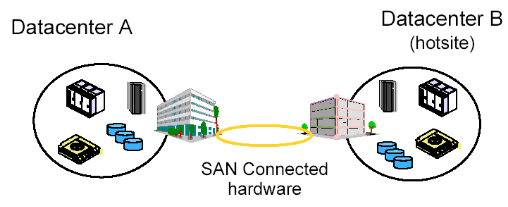
\includegraphics[width=8cm]{tier4.png}
\caption{Tier 4 \href{https://www.abzsol.com/cms/images/stories/pdf/business_continuity.pdf}{www.abzsol.com}}\end{figure}
Per SAP è previsto:
\begin{itemize}
\item backup off-site radicale ogni sei mesi su nastro  da conservare presso l'\textit{Offerente};
%\item backup off-site incrementale una volta al giorno su disco;
\item SAN connected hardware;
%\item backup off-site radicale ogni sei mesi su nastro;
%\item backup off-site incrementale una volta al giorno su disco;
%\item electronic vaulting per i dati più critici;
\item software di gestione Disaster Recovery (da stabilire in progettazione esecutiva - es: VMware che ben si integra con SAP e che supporta le SAN);
\item hot-site con installazione dei sistemi SAP (con relative librerie e documentazione);
\end{itemize}
Dovrà essere scelto un software di Disaster Recovery specifico per SAP, da integrare col software di gestione di DR degli altri sistemi presenti nella soluzione, con possibilità di personalizzazione di parametri quali la frequenza e la modalità di backup: la perdita di alcune ore di dati è ancora ammissibile, ma copie di tipo Point-in-Time (PIT) permettono con falicità backup con una frequenza più elevata rispetto al semplice trasferimento dei dati su nastro.
Quindi, anche se i dati potrebbero essere aggiornati nel peggiore dei casi alle 4 ore precedenti, i sistemi sostitutivi saranno già funzionanti.
Altri dati necessari per eseguire l'applicazione (librerie, documentazione, copie delle licenze software) vengono inviati anche al sito secondario attraverso il software di gestione del DR al momento della creazione della soluzione. Il software permetterà anche il monitoraggio e il controllo della situazione in ogni momento sia antecedente all'emergenza, sia in fase di emergenza, che di rientro.

\subsubsection{Fase di reazione all’emergenza}
Istruzioni operative del start-up di dettaglio verranno fornite in sede di progettazione esecutiva. Si cercherà di automatizzare al massimo ogni operazione tramite script automatici, di modo da minimizzare, per quanto possibile, l'intervento umano. 
Supponendo che strutture generali, infrastruttura e componenti hardware siano ripristinati, le procedure di recupero rispetteranno le seguenti linee guida generali:
\begin{itemize}
\item avvio dei sistemi nel sito secondario tramite software di gestione del DR;
\item lancio della riconfigurazione automatizzata delle risorse di rete;
\item controllo del corretto collegamento del sistema alla rete di produzione;
\item controllo del corretto ripristino dei sistemi operativi;
\item ripristino dei dati applicativi;
\item controllo del corretto ripristino della configurazione dei dati di sistema;
\item controllo del corretto ripristino del software applicativo;
\item lancio del testing automatizzato per la sicurezza;
\item lancio del testing automatizzato per le funzionalità di base del sistema;
\end{itemize}

\subsubsection{Fase di gestione dell’emergenza}
\begin{itemize}
\item L'amministrazione e monitoraggio dei sistemi di sostituzione per SAP viene affidato all'ing. X, e in secondo luogo al sig. XX.
\item Non è previsto che gli operatori sanitari, amministrativi, o che i tecnici debbano spostarsi fisicamente verso la struttura sostitutiva.
\item La situazione sarà sempre controllabile da remoto sia dall'Istituto che dalla \textit{nostra} azienda.
\item In caso di necessità è prevista la possibilità di mandare tecnici della \textit{nostra} azienda o professionisti esterni mandati da parte della nostra azienda.
\item Gli accessi si sistemi SAP dovranno essere controllati dal software di gestione di DR.
\item I dati creati in fase di gestione dell'emergenza devono essere memorizzati in un ambiente secondario, in modo da facilitarne il successivo restore.
\end{itemize}


%*************************************************************
\newpage
\subsection{Soluzione di Continuità per SISS}
\subsubsection{Interrelazioni con entità esterne all’Amministrazione}
I contratti in essere che vengono coinvolti sono:
\renewcommand \arraystretch{1,5}
\begin{longtable}{c c c}
\toprule
\textbf{Contratto in Essere} & \textbf{Fornitore} & \textbf{Produttore} \\
\toprule
	Contratto unico per fornitura servizi IT & Offerente & Offerente \\
\bottomrule
\caption{Contratti SISS}
\end{longtable}
Non si rilevano necessità di effettuare variazioni contrattuali ai contratti sopracitati.
\subsubsection{Assunzioni ai fini del progetto didattico}
Ai fini del progetto didattico,si suppone che i dati che vengono creati all'interno dell'Istituto siano memorizzati nelle repository centrali oppure che vengano spediti ai server centrali SISS, e che quindi nella \textit{"Porta Applicativa"} esistano server, routers, firewall e il software atti all'invio e alla ricezione di dati da e verso i DB centrali SISS, senza vere e proprie strutture ospitanti dati al suo interno. Si specifica che, anche in caso questa assunzione sia scorretta, sarebbe stata ipotizzata una soluzione simile a quella indicata successivamente per i servizi SAP.
\subsubsection{Soluzione}
Per SISS è prevista l'adozione del Tier 4 con:
\begin{itemize}
\item software di gestione Disaster Recovery (da stabilire in progettazione esecutiva es: Tivoli IBM);
\item warm-site con
  \begin{itemize}
  \item installazione della \textit{Porta Applicativa SISS} (con relative librerie e documentazione);
  \item cache predisposta per la memorizzazione temporanea delle richieste verso i sistemi centrali SISS;
  \end{itemize}
\end{itemize}
Saranno presenti le attrezzature hardware dotate di connessione e pre-configurate. In caso di emergenza verrà come prima cosa avviata la cache temporanea, che servirà per la presa in carico delle richieste verso i sistemi centrali SISS. Queste richieste verranno gestite una volta che il servizio sostitutivo sarà attivo. L'attivazione della soluzione sostitutiva nel frattempo sarà gestita attraverso il software di gestione di DR prescelto.
\\
Altri dati necessari per eseguire l'applicazione (librerie, documentazione, copie delle licenze software) vengono inviati anche al sito secondario attraverso il software di gestione del DR al momento della creazione della soluzione. Il software permetterà anche il monitoraggio e il controllo della situazione in ogni momento sia antecedente all'emergenza, sia in fase di emergenza, che di rientro.

\subsubsection{Fase di reazione all’emergenza}
Istruzioni operative del start-up di dettaglio verranno fornite in sede di progettazione esecutiva. Si cercherà di automatizzare al massimo ogni operazione tramite script automatici, di modo da minimizzare, per quanto possibile, l'intervento umano. 
Supponendo che strutture generali, infrastruttura e componenti hardware siano ripristinati, le procedure di recupero rispetteranno le seguenti linee guida generali:
\begin{itemize}
\item avvio della cache temporanea tramite software di gestione del DR;
\item avvio dei sistemi sostitutivi tramite software di gestione del DR;
\item lancio della riconfigurazione automatizzata delle risorse di rete;
\item collegamento del sistema alla rete di produzione;
\item ripristino dei sistemi operativi;
\item lancio del testing automatizzato per la sicurezza;
\item lancio del testing automatizzato per le funzionalità di base del sistema;
\item gestione delle richieste accodate nella cache temporanea;
\end{itemize}

\subsubsection{Fase di gestione dell’emergenza}
\begin{itemize}
\item L'amministrazione e monitoraggio dei sistemi di sostituzione per la \textit{Porta Applicativa SISS} viene affidato all'ing. X, e in secondo luogo al sig. XX.
\item Non è previsto che gli operatori sanitari, amministrativi, o che i tecnici debbano spostarsi fisicamente verso la struttura sostitutiva.
\item La situazione sarà sempre controllabile da remoto sia dall'Istituto che dalla \textit{nostra} azienda.
\item In caso di necessità è prevista la possibilità di mandare tecnici della \textit{nostra} azienda o professionisti esterni mandati da parte della nostra azienda.
\item Gli accessi si sistemi appartenenti alla \textit{Porta Applicativa SISS} dovranno essere controllati dal software di gestione di DR.
\end{itemize}

%***************************************************

\newpage
\subsection{Fase di ritorno alla normalità}
\label{rientro}
Il software di gestione di DR deve gestire in modo più automatizzato possibile tutte le operazioni di rientro dalla situazione di emergenza. In particolare ci si aspetta che i dati creati in fase di gestione dell'emergenza saranno trasferiti in fase di  verso l'Istituto utilizzando procedure automatizzate.
Istruzioni operative del restore di dettaglio verranno fornite in sede di progettazione esecutiva. Supponendo che le funzioni di supporto dell'infrastruttura (alimentazione,  telecomunicazioni, strutture fisiche e hardware) siano stati correttamente riportati alla normalità, le procedue di restore rispetteranno le seguenti linee guida generali:
\begin{itemize}
\item controllo della corretta installazione dell'hardware;
\item ripristino del software di sistema;
\item ripristino del software applicativo;
\item ripristino dei dati sui sistemi di produzione;
\item controllo del corretto ripristino della configurazione dei dati di sistema;
\item lancio della riconfigurazione automatizzata delle risorse di rete;
\item avvio dei sistemi primari;
\item lancio del testing automatizzato per la sicurezza;
\item lancio del testing automatizzato per le funzionalità di base del sistema;
\item test per le funzionalità non di base del sistema;
\item arresto delle operazioni di emergenza;
\item reset e riconfigurazione del software di gestione del DR;
\item reset e riconfigurazione dei sistemi secondari.
\end{itemize}

Una volta che l'infrastruttura, la rete, i sistemi, le applicazioni e le interfacce sono stati testati per la produzione, il sito primario torna allo stato ordinario e il sito secondario viene riconfigurato di modo che sia pronto per reagire a un'eventuale futuro stato di emergenza. Infine le misure di emergenza verranno riviste in un ottica di miglioramento, come descritto in \textit{Operational Management} in \ref{opmgmt}. Entro un mese dal rientro della situazione di emergenza deve essere stilata la reportistica apposita contenente:
\begin{itemize}
\item descrizione dell'emergenza
\item analisi dei danni;
\item report attivazione gestione e rientro;
\item descrizione test di verifica rientro.
\end{itemize}















































%*******************************************************
\newpage
\section{Operational Management}
\label{opmgmt}
Una volta che l'implementazione e la pianificazione sono completate è necessario garantire che il processo sia mantenuto come parte del normale business.
\subsection{Education and Awareness} Tutto l'Istituto e in modo particolare i dipartimenti IT sono chiamati alla piena comprensione delle motivazioni che spingono verso l'adozione di misure di Continuità, in modo che siano al corrente delle implicazioni della Continuity nel loro lavoro quotidiano.
A tale scopo l'IT SC Manager organizzarà una volta all'anno nel mese di XX un seminario della durata di due ore.
\subsection{Formazione}
È importante garantire che il personale IT sia sempre competente e autonomo per quanto riguarda la Continuità. E' necessario quindi:
\begin{itemize}
\item stendere una documentazione appropriata che descriva la soluzione di continuità comprendendo ogni attività che i membri del team devono fare, le modalità e le tempistiche, assieme ai ruoli che devono assumere e le loro responsabilità;
\item tenere seminari sia di carattere teorico che pratico per assicurare la piena comprensione dei contenuti: sono previste 24 ore di formazione al termine del progetto e 8 ore di formazione ogni anno. Le modalità saranno concordate nel dettaglio in fase di progettazione esecutiva.
\item tenere verifiche annuali al termine dei seminari. Le modalità saranno concordate nel dettaglio in fase di progettazione esecutiva.
\end{itemize}
\subsection{Modalità di esecuzione dei test periodici}
Per quanto attiene ai test sono possibili varie modalità di test: 
\begin{itemize}
\item \textbf{checklist}: viene effettuata una semplice verifica dell’effettiva disponibilità di tutto quanto si renderebbe necessario in caso di emergenza, basandosi su una cheklist, come descritto nella sezione successiva;
\item \textbf{test  degli  impianti  e  delle  risorse con sistemi primari attivi: } Il Responsabile per la Continuità avvierà l'esecuzione della simulazione che coinvolgerà l'attivazione  delle  risorse  fisiche secondarie, senza la disattivazione delle risorse primarie. Durante la simulazione per ognuna delle fasi, vengono eseguite le attività previste nel corrente piano e il Responsabile monitorerà attentamente l'esecuzione fino a quando i servizi non saranno tornati alla normalità.
\item \textbf{test  degli  impianti  e  delle  risorse con disattivazione dei sistemi primari:}  viene effettuata una simulazione che coinvolga l’effettiva 
attivazione  delle  risorse  fisiche  e  IT e, per ognuna delle fasi, vengono eseguite le attività previste nel corrente piano e una verifica dell'uso delle corrette procedure. Per Aurora è previsto che, durante la disattivazione, venga usato l'ambiente di test. Il Responsabile per la Continuità avvierà l'esecuzione del piano e monitorerà attentamente l'esecuzione fino a quando i servizi non saranno tornati alla normalità. Un  test  di  questo  tipo  richiede  una  attenta  predisposizione  e  un  sensibile impegno  per  il  personale,  ma  garantisce  la  reale  verifica  della  soluzione  di  continuità  del  PCO  ICT. 
\end{itemize}
In caso di errori o incompletezze, il piano viene rivisitato come descritto nella sezione seguente.
I test vanno eseguiti dopo ogni eventuale calamità che dovesse attivare qualche soluzione di emergenza.
\subsubsection{Frequenza e finestre per i test}
\begin{itemize}
\item simulazione in attivo: 1 volta all'anno - durante il mese di MeseX dalle hh:mm alle hh:mm, senza preavviso del personale;
\item checklist: 1 volta all'anno - entro un mese dopo la simulazione in attivo;
\item simulazione con disattivazione: 1 volta all'anno da concordare entro il GG Mese+1, e da effettuare con un preavviso di almeno 1 mese.
\end{itemize}
E' necessario un documento scritto o elettronico che attesti l'esecuzione di ogni test.
\subsection{Modalità di revisione e adeguamento del piano}
Il Piano di Continuità ICT non è un documento statico e, pertanto, è necessario pianificare, all’interno del PCO ICT stesso le modalità di revisione e aggiornamento. Sarà il SC team ad effettuare la revisione, guidato dall'IT SC Manager.
La modalità di revisione è scelta è la \textit{checklist}, un elenco di punti da controllare da predisporre nel dettaglio in fase di progettazione esecutiva, ma che in linea di massima conterrà i punti relativi a:
  \begin{itemize}
  \item modifiche nella composizione della/e struttura/e organizzava/e preposte alla gestione della continuità operativa ICT; 
  \item modifiche nei dati personali e/o di reperibilità;
  \item modifiche dei fornitori e/o del contratto assicurativo; 
  \item modifiche dei servizi o delle applicazioni software (aggiunta o eliminazione di applicazioni, 
  variazioni nella criticità/priorità delle applicazioni); 
  \item modifiche nell’hardware e/o nella rete;
  \item modifiche nella logistica; 
  \item stipula di nuovi contratti. 
  \end{itemize}
  Vista la natura della checklist, il Service Continuity Team sarà chiamato a collaborare con il Change Management per una armonizzazione di quanto descritto tra i due processi di Change e Continuity. In particolare ad ogni cambiamento che avverrà a uno dei punti stabiliti nella check-list è previsto che sia il Change Management che in maniera attiva informi il Service Continuity Team. Al termine di ogni revisione del presente documento, le Change opportune devono essere gestite assieme al CAB.
Il corrente piano viene rivisitato secondo la modalità descritta dal Comitato di Revisione e approvato dal Responsabile della Continuità ICT.